\documentclass[8pt]{article}
\usepackage[UTF8]{ctex}
\usepackage[a4paper]{geometry}

\usepackage{amsthm,amsmath,amssymb}
\usepackage{graphicx}
\usepackage{subfigure}
\usepackage{amsmath}
\usepackage{tabularx}
\usepackage{color}
\usepackage{hyperref}
\usepackage{ulem}
\usepackage{multirow}
\usepackage[cache=false]{minted}
\hypersetup{
	colorlinks=True,
	linkcolor=blue
}

\usepackage{appendix}
\geometry{a4paper,centering,scale=0.8}
\geometry{left=2.0cm, right=2.0cm, top=2.5cm, bottom=2.5cm}
\usepackage[format=hang,font=small,textfont=it]{caption}
\usepackage[nottoc]{tocbibind}

\usepackage{algorithm}
\usepackage{algorithmicx}
\usepackage{algpseudocode}
\usepackage{amssymb}
\usepackage{extarrows}
\usepackage{qcircuit}
\usepackage{fancyhdr}
\usepackage{fancyvrb}

\fvset{showspaces=True}
\SaveVerb{verbspace}! !
\newcommand{\aspace}{\UseVerb{verbspace}}%
\usepackage{cleveref}

\usepackage{pgf}
\usepackage{totpages}
\usepackage{tikz}  
\usetikzlibrary{arrows,automata}

\usetikzlibrary{arrows.meta}%画箭头用的包

\makeatletter
\def\@maketitle{%
	\newpage
	\begin{center}%
		\let \footnote \thanks
		{\LARGE \@title \par}%
		\vskip 1.5em%
		{\large
			\lineskip .5em%
			\begin{tabular}[t]{c}%
				\@author
			\end{tabular}\par}%
		\vskip 1em%
		{\large \@date}%
	\end{center}%
	\par
	\vskip 1.5em}
\makeatother

\newtheoremstyle{compact}%
{3pt}{3pt}%
{}{}%
{\bfseries}{\textcolor{red}{.}}%  % Note that final punctuation is omitted.
{.5em}{\mbox{\textcolor{red}{\thmname{#1}\thmnumber{ #2}}\thmnote{ (\textcolor{blue}{#3})}}}
\theoremstyle{compact}
\newtheorem{innercustomgeneric}{\customgenericname}
\providecommand{\customgenericname}{}
\newcommand{\newcustomtheorem}[2]{%
	\newenvironment{#1}[1]
	{%
		\renewcommand\customgenericname{#2}%
		\renewcommand\theinnercustomgeneric{##1}%
		\innercustomgeneric
	}
	{\endinnercustomgeneric}
}

\DeclareMathOperator{\card}{card}

\newtheorem{theorem}{定理}[section]
\newtheorem{lemma}{引理}[section]
\newtheorem{definition}{定义}[section]
\newtheorem{proposition}{命题}[section]
\newtheorem{corollary}{推论}[section]
\newtheorem{example}{例}[section]
\newtheorem{claim}{断言}[section]
\newtheorem{remark}{注}[section]
\newtheorem{thesis}{论点}[section]
\newtheorem{Proof}{证明}

\def\obj#1{\textbf{\uline{#1}}}
\def\num#1{\textnormal{\textbf{\mbox{\textcolor{blue}{(#1)}}}}}
\def\le{\leqslant}
\def\ge{\geqslant}
\def\im{\text{im }}
\def\Pr#1{\text{Pr}\left[{#1}\right]}
\def\E#1{\mathbb{E}\left[{#1}\right]}
\def\Var#1{\text{Var}\left[{#1}\right]}
\def\rep#1{\llcorner{#1}\lrcorner}

\def\DTIME{\textbf{DTIME}}
\def\NTIME{\textbf{NTIME}}
\def\P{\textbf{P}}
\def\NP{\textbf{NP}}
\def\coNP{\textbf{coNP}}
\def\EXP{\textbf{EXP}}
\def\NEXP{\textbf{NEXP}}
\def\SPACE{\textbf{SPACE}}
\def\NSPACE{\textbf{NSPACE}}
\def\PSPACE{\textbf{PSPACE}}
\def\NPSPACE{\textbf{NPSPACE}}
\def\L{\textbf{L}}
\def\NL{\textbf{NL}}
\def\coNL{\textbf{coNL}}

\def\PH{\textbf{PH}}

\def\SIZE{\textbf{SIZE}}
\def\PPOLY{$\textbf{P}_{\textbf{/poly}}$}
\def\NC{\textbf{NC}}
\def\AC{\textbf{AC}}

\def\BPTIME{\textbf{BPTIME}}
\def\BPP{\textbf{BPP}}
\def\coBPP{\textbf{coBPP}}

\def\RTIME{\textbf{RTIME}}
\def\RP{\textbf{RP}}
\def\coRP{\textbf{coRP}}
\def\ZTIME{\textbf{ZTIME}}
\def\ZPP{\textbf{ZPP}}

\title{\heiti\zihao{1} 计算理论导论\ 课程笔记}
\author{\kaishu\zihao{-3} 酥雨\\zusuyu@stu.pku.edu.cn}

\CTEXoptions[today=old]
\date{\today}

\begin{document}
\fancypagestyle{plain}{
	\fancyhf{}
	\lhead{计算理论导论\ 课程笔记}
	\chead{\today}
	\rhead{TCS notes}
	\cfoot{第 \thepage 页, 共 \pageref{TotPages} 页}
}
\pagestyle{plain}

\crefname{definition}{定义}{定义}
\crefname{theorem}{定理}{定理}
\crefname{lemma}{引理}{引理}
\crefname{proposition}{命题}{命题}
\crefname{remark}{注}{注}
\crefname{figure}{图}{图}
\crefname{table}{表}{表}	
\maketitle
\tableofcontents
\iffalse
\section*{Outline}
	\begin{enumerate}	
		\item DFA/NFA, Regular Language, Pumping Lemma
		\item Context-free Language, Pumping Lemma
		\item Turing Machine
		\item Undecidable Language
		\item Time Complexity \P\ and \NP
		\item Space Complexity \PSPACE, \L\ and \NL
		\item Polynomial Hierarchy
		\item Circuit Complexity
		\item Random Computation
		\item Interactive Proof
		\item (optional) Crypt, Quant, Learning
	\end{enumerate}
\fi


\newpage
\section{正则语言}
\subsection{有限自动机}
\begin{definition}[Deterministic Finite Automaton, DFA]
	(确定性)有限自动机是一个五元组$(Q, \Sigma, \delta, q_0, F)$, 其中
	\begin{itemize}
		\item $Q$是称为\obj{状态}的有限集. 
		\item $\Sigma$是称为\obj{字符集}的有限集. 
		\item $\delta: Q \times \Sigma \to Q$被称为\obj{转移函数}. 
		\item $q_0 \in Q$称为\obj{起始态}. 
		\item $F \subseteq Q$称为\obj{接受态(终止态)集合}. 
	\end{itemize}

	称字符串$w = w_1w_2\cdots w_m(w_i \in \Sigma)$可以被DFA $M = (Q, \Sigma, \delta, q_0, F)$接受, 如果存在状态序列$r_0, r_1, \cdots, r_m \in Q$满足\num{i}$r_0 = q_0$, \num{ii}$r_{i+1} = \delta(r_i, w_{i+1}) \ (\forall i = 0, 1, \cdots, m-1)$, \num{iii}$r_m \in F$. 

	所有可被$M$识别的字符串$w$构成集合$A$, 则称$A$是 DFA $M$的语言(或者说 DFA $M$识别/接受$A$), 记为$L(M) = A$.
\end{definition}
\begin{definition}[正则语言]
	正则语言就是能够被有限自动机识别的语言. 
\end{definition}
\begin{definition}[正则操作]
	定义如下三种正则操作
	\begin{itemize}
		\item \obj{Union}: $A \cup B = \{x | x \in A \textrm{ or } x \in B\}$.
		\item \obj{Concatenation}: $A \circ B = \{xy | x \in A \textrm{ and } y \in B\}$.
		\item \obj{Star}: $A^* = \{x_1x_2\cdots x_k | k \ge 0 \textrm{ and each } x_i \in A\}$.
	\end{itemize}
\end{definition}
\begin{remark}
	补集$\overline{A} = \Sigma^* - A$操作在正则语言下是封闭的: 只需要把终止态集合$F$改成$Q - F$即可.
\end{remark}
\begin{theorem}
	正则操作 union 在正则语言下是封闭的: 把两个自动机放在一起跑就行了. 
\end{theorem}
由于只利用已有的有限自动机模型证明 concatenation 和 star 的封闭性是困难的, 我们引入“非确定性”. 
\begin{definition}[Nondeterministic Finite Automaton, NFA]
	非确定性有限自动机是一个五元组$(Q, \Sigma, \delta, q_0, F)$, 其中$\delta$不再是$Q \times \Sigma \to Q$的函数, 而是$Q \times \Sigma_{\varepsilon} \to \mathcal P(Q)$的, 其中$\mathcal P$表示幂集, $\Sigma_{\varepsilon}$表示$\Sigma \cup \{\varepsilon\}$. 

	相应的, 称字符串$w = w_1w_2\cdots w_m(w_i \in \Sigma)$可以被NFA $N = (Q, \Sigma, \delta, q_0, F)$接受, 如果$w$可以写成$w = y_1y_2\cdots y_{m'}(y_i \in \Sigma_{\varepsilon})$, 且存在状态序列$r_0, r_1, \cdots, r_{m'} \in Q$满足\num{i}$r_0 = q_0$, \num{ii}$r_{i+1} \in \delta(r_i, y_{i+1})$\ $(\forall i = 0, 1, \cdots, {m'}-1)$, \num{iii}$r_{m'} \in F$. 
\end{definition}
\begin{remark}
	DFA的每个状态对每种字符都有恰好一条转移出边, 而相对的, NFA可能有零条、一条或者多条, 有几条出边就表示会创建出多少个独立的“后继进程”. 此外还存在$\varepsilon$的出边, 表示可以不输入任何字符创建进程. 
\end{remark}
\begin{theorem}[NFA与DFA的等价性]
	任何NFA都存在等效的DFA. 
\end{theorem}
\begin{proof}
	对$k$个状态的NFA, 构造一个$2^k$个状态的DFA, 每个状态表示“可能处在的NFA状态”的子集. 

	形式化的, 对于 NFA $M = (Q, \Sigma, \delta, q_0, F)$, 构造 DFA $M' = (Q', \Sigma, \delta', q_0', F')$, 其中
	\begin{itemize}
		\item $Q' = \mathcal P(Q)$.
		\item $\forall R \in Q', a \in \Sigma, \delta'(R, a) = \bigcup_{r \in R}\delta(r, a)$.
		\item $q_0' = \{q_0\}$.
		\item $F' = \{R \in Q' | R \cap F \neq \varnothing\}$.
	\end{itemize}
\end{proof}
\begin{corollary}
	一个语言是正则的当且仅当可以被一台非确定性有限自动机识别. 
\end{corollary}
\begin{theorem}
	union, concatenation 和 star 在正则语言下都是封闭的. 
\end{theorem}
\begin{proof}
	不多说了看图. 

	\begin{figure}[htbp]
		\centering
		\subfigure[proof for union]{
			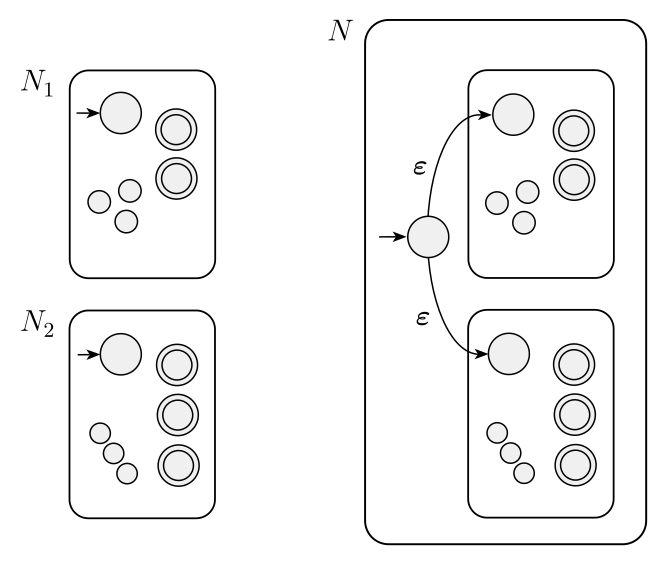
\includegraphics[scale=0.25]{pic/union.png}
		}
		\quad
		\subfigure[proof for concatenation]{
			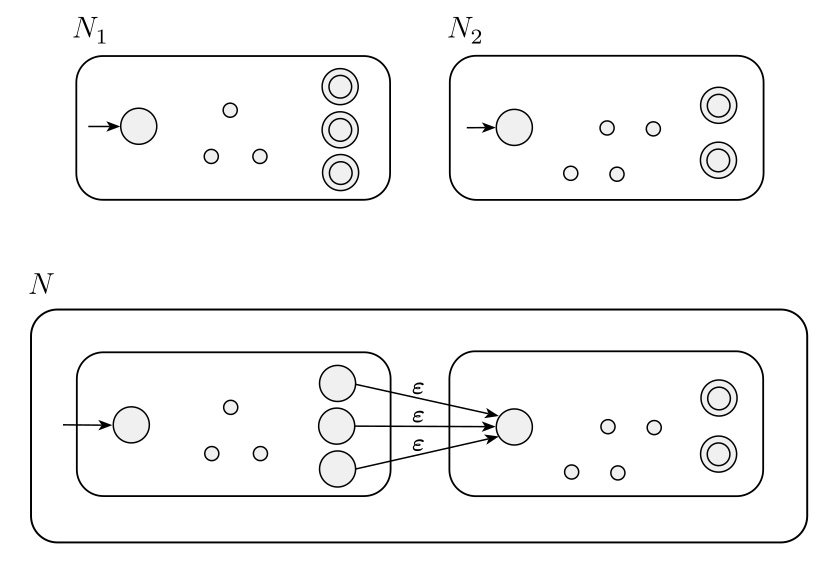
\includegraphics[scale=0.25]{pic/concat.png}
		}
		\quad
			\subfigure[proof for star]{
			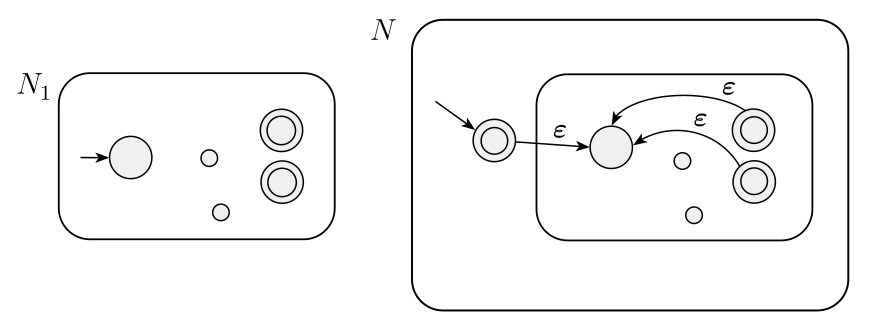
\includegraphics[scale=0.25]{pic/star.png}
		}
	\end{figure}
\end{proof}
\subsection{正则表达式}
\begin{definition}[正则表达式]
	称$R$是正则表达式, 如果$R$为
	\begin{itemize}
		\item $\{a\}$, 其中$a$是字符集$\Sigma$中的某个元素
		\item $\{\varepsilon\}$, 其中$\varepsilon$表示空串
		\item $\varnothing$
		\item $(R_1 \cup R_2)$, 其中$R_1, R_2$是某两个正则表达式
		\item $(R_1 \circ R_2)$, 其中$R_1, R_2$是某两个正则表达式
		\item $(R_1^*)$, 其中$R_1$是某个正则表达式
	\end{itemize}
\end{definition}
\begin{example}
	对于任意正则表达式$R$, $R \cup \varnothing = R \circ \varepsilon = R$, $R \circ \varnothing = \varnothing$, $\varnothing^* = \{\varepsilon\}$. 
\end{example}
\begin{theorem}[正则表达式与有限自动机的等价性]
	一个语言是正则的当且仅当它可以被一个正则表达式描述. 
\end{theorem}
\begin{proof}
	“$\Leftarrow$”的证明是简单的, 只需要根据正则表达式$R$构造NFA, 利用“union, concatenation, star的封闭性”的构造性证明即可. 

	“$\Rightarrow$”的证明中, 我们引入GNFA的定义(每条转移边上的label是一个正则表达式), 然后分别展示如何把DFA转化成GNFA以及如何根据GNFA构造正则表达式. 

	DFA转GNFA是简单的——只需要额外加入两个状态表示$q_{\text{start}}$和$q_{\text{accept}}$即可. 

	观察到一个GNFA有$k \ge 2$个状态. 如果$k=2$, 那么$q_{\text{start}}$到$q_{\text{accept}}$的转移边上的正则表达式就是该有限自动机对应的正则表达式. 如果$k > 2$, 那么考虑选出一个状态$q_{\text{rip}}$删除, 此时对于$q_i, q_j \in Q \setminus \{q_{\text{rip}}\}$, 如果$\delta(q_i,  q_{\text{rip}}) = R_1, \delta(q_{\text{rip}}, q_{\text{rip}}) = R_2, \delta(q_{\text{rip}}, q_j) = R_3, \delta(q_i, q_j) = R_4$, 则修改$\delta'(q_i, q_j) = (R_1)(R_2)^*(R_3) \cup (R_4)$. 归纳即可. 
\end{proof}
\begin{definition}[Generalized Nondeterministic Finite Automaton, GNFA]
	广义非确定性有限自动机是一个五元组$(Q, \Sigma, \delta, q_{\text{start}}, q_{\text{accept}})$, 其中$\delta$是$(Q \setminus \{q_{\text{accept}}\}) \times (Q \setminus \{q_{\text{start}}\}) \to \mathcal R$的转移函数, $\mathcal R$表示字符集$\Sigma$上的所有正则表达式. 注意不失一般性地要求了只有唯一的接受态, 以及$q_{\text{start}} \neq q_{\text{accept}}$. 
\end{definition}
\subsection{Pumping Lemma}
\begin{theorem}[Pumping Lemma for Regular Language]
	如果$A$是正则语言, 那么存在一个数$p$ (称为\obj{pumping length}), 使得对于任意$A$中长度至少为$p$的字符串$s$, $s$都可分成三部分$s = xyz$满足
	\begin{itemize}
		\item for each $i \ge 0$, $xy^iz \in A$,
		\item $|y| > 0$,
		\item $|xy| \le p$.
	\end{itemize}
\end{theorem}
\begin{proof}
	取 pumping length $p$ 为识别此正则语言的 DFA $M$的状态集大小$|Q|$. 对于任意长度至少为$p$的$s \in A$, 其经过的状态序列至少长为$p+1$. 根据\obj{鸽巢原理}, 存在一个状态$q$经过了至少两次, 于是把从$q_{\text{start}}$走到$q$的部分视作$x$, $q$回到自身的环视作$y$, 从$q$走到$q_{\text{accept}}$的部分视作$z$, 便构造出了划分. 
\end{proof}
\begin{remark}
	利用 pumping lemma 可以证明某个语言$B$不是正则语言, 通用的方式是:先假设$B$是正则的, 导出 pumping length $p$的存在性, 然后根据这个$p$构造$s \in B$, 并验证其\obj{不能}被划分为$s = xyz$. 第三个条件$|xy| \le p$有时也是有用的. 
\end{remark}
\begin{example}
	$B = \{0^n1^n | n \ge 0\}$ 不是正则语言.
\end{example}
\begin{proof}
	假设 $B$ 是正则语言, 那么就存在 pumping length $p$. 考虑串 $0^p1^p$, 无论 $y$ 取其何种子串, $xyyz$ 都不可能 $\in B$. 因此 $B$ 不是正则语言.
\end{proof}
\begin{example}
	$C = \{w | w \text{ has an equal number of 0s and 1s}\}$ 不是正则语言.
\end{example}
\begin{proof}
	假设 $C$ 是正则语言, 那么就存在 pumping length $p$. 考虑串 $0^p1^p$, 注意到我们要求了 $|xy| \le p$, 所以 $y$ 只能包含 $0$, 此时 $xyyz \notin B$. 因此 $C$ 不是正则语言.
	
	\textit{另一种证法是: 考虑 $C \cap 0^*1^* = B$, 正则语言在 intersection 下是封闭的, 所以$C$正则会导出$B$正则.}
\end{proof}
\begin{example}
	$F = \{ww | w \in \{0, 1\}^*\}$ 不是正则语言.
\end{example}
\begin{proof}
	考虑串 $0^p10^p1$, 注意到 $y$ 只能包含 $0$, 从而$xyyz \notin F$, 因此$F$不是正则语言.
\end{proof}

\begin{example}
	$D = \{1^{n^2} | n \ge 0\}$ 不是正则语言.
\end{example}
\begin{proof}
	考虑串 $1^{p^2}$. 由于 $|y| \le p$, 所以 $|xyyz| = p(p+1) < (p+1)^2$ 不可能是完全平方数, $xyyz \notin D$, 说明$D$不是正则语言.
\end{proof}
\begin{example}
	$E = \{0^i1^j | i > j\}$不是正则语言. 
\end{example}
\begin{proof}
	考虑串$0^{p+1}1^p$, $y$只能包含 $0$, 且$|y| > 0$, 因此$xz$中$0$的个数不超过 $1$的个数, $xz \notin E$, 说明 $E$ 不是正则语言.
\end{proof}
\newpage
\section{上下文无关语言}
\subsection{上下文无关文法}
\begin{definition}[Context-Free Grammar/Language, CFG/CFL]
	一个上下文无关文法是一个四元组$(V, \Sigma, R, S)$, 其中
	\begin{itemize}
		\item $V$是称为\obj{变量}的有限集, 
		\item $\Sigma$是称为\obj{终止符}的有限集, 与$V$不交, 
		\item $R$是称为\obj{规则}的有限集, 是从$V$到$(V \cup \Sigma)^*$的映射, 
		\item $S \in V$称为\obj{起始变量}. 
	\end{itemize}

	上下文无关语言就是上下文无关文法导出/生成的语言, 即$\{w \in \Sigma^* | S \overset{*}{\Rightarrow} w\}$. 
\end{definition}
\begin{definition}[parse tree]
	形如这样子的东西.
	\begin{center}
		\includegraphics*[scale=0.4]{pic/parse_tree.png}	
	\end{center}
\end{definition}
\begin{proposition}
	CFG 的描述能力严格强于有限自动机(或者正则表达式). 
\end{proposition}
\begin{proof}
	对于任意的DFA, 都可以构造与其等价的CFG:对每个状态$q_i$构造一个变量$R_i$, 起始变量$R_0$对应起始态$q_0$, 如果$\delta(q_i, a) = q_j$, 就添加规则$R_i \to aR_j$, 而如果$q_i$是接受态, 就添加规则$R_i \to \varepsilon$. 

	而显然存在可被 CFG 描述的非正则语言, 比如$\{0^n1^n | n \in \mathbb N\}$. 
\end{proof}
\begin{definition}[歧义性]
	称一个串 $w$ 由 CFG $G$ 歧义生成, 如果存在 $G$ 下 $w$ 的两种 lestmost derivation (每次只替换最左边的变量)方式, 或者说存在两棵不同的 parse tree 可以生成 $w$. 称一个 CFG $G$ 是歧义的, 如果它可以歧义生成某些串.
\end{definition}
\begin{definition}[固有歧义]
	称一个 CFL $L$ 是固有歧义的, 如果 $L$ 只能由歧义的 CFG $G$ 生成.
\end{definition}
\begin{example}
	$\{a^ib^jc^k | i = j \textrm{ or } j = k\}$ 是固有歧义的.
\end{example}

\subsection{下推自动机}

我们希望能给有限自动机做一些加强, 使其能够达到与 CFG 相同的表达能力. 最终决定了为其添加栈结构, 于是得到了如下定义的“下推自动机”:

\begin{definition}[Pushdown Automaton, PDA]
	下推自动机是一个六元组$(Q, \Sigma, \Gamma, \delta, q_0, F)$, 其中
	\begin{itemize}
		\item $Q$是状态集, 
		\item $\Sigma$是输入字符集, 
		\item $\Gamma$是栈字符集, 
		\item $\delta: Q \times \Sigma_{\varepsilon} \times \Gamma_{\varepsilon} \to \mathcal P(Q \times \Gamma_{\varepsilon})$是转移函数, 
		\item $q_0 \in Q$是起始态, 
		\item $F \subseteq Q$是接受态集合. 
	\end{itemize}

	其中$\Sigma_{\varepsilon}, \Gamma_{\varepsilon}$分别表示$\Sigma \cup \{\varepsilon\}, \Gamma \cup \{\varepsilon\}$. $(q', b) \in \delta(q, c, a)$ 表示在状态 $q$ 上被输入 $c$ 字符时, 会先从栈顶 pop 出字符 $a$, 再向栈顶 push 进字符 $b$, 最后转移到状态 $q'$. 幂集$\mathcal P$暗含了下推自动机是 nondeterministic 的. 

	称字符串$w = w_1w_2\cdots w_m(w_i \in \Sigma_{\varepsilon})$可以被 PDA $M = (Q, \Sigma, \Gamma, \delta, q_0, F)$接受, 如果存在状态序列$r_0, r_1, \cdots, r_m \in Q$和字符串(栈)序列$s_0, s_1, \cdots, s_m \in \Gamma^*$, 满足
	\begin{itemize}
		\item $r_0 = q_0, s_0 = \varepsilon$,
		\item for $i = 0, 1, \cdots, m-1$, $(r_{i+1}, b) \in \delta(r_i, w_{i+1}, a)$, where $s_i = at, s_{i+1}=bt$ for some $a, b \in \Gamma_{\varepsilon}$ and $t \in \Gamma^*$,
		\item $r_m \in F$.
	\end{itemize}

	类似的, 可以定义 $L(M)$ 表示 PDA $M$ 接受的所有字符串构成的集合, 即 $M$ 所识别的语言.
\end{definition}

\begin{theorem}[下推自动机与上下文无关文法的等价性]
	一个语言是上下文无关的, 当且仅当存在某个下推自动机可以识别它. 
\end{theorem}
\begin{proof}
	“$\Rightarrow$”: 需要根据 CFG 来构造 PDA. 一开始把 CFG 的起始变量写在栈上, 并保证在替换过程中栈顶始终是一个尚未替换的变量. 利用 nondeterminism 尝试每一种变量的替换方式. 每次只考虑替换栈顶的变量, 而如果栈顶是一个终止符, 就直接和输入匹配掉. 当输入匹配完且栈为空时, 代表输入串可接受. 

	\begin{center}
		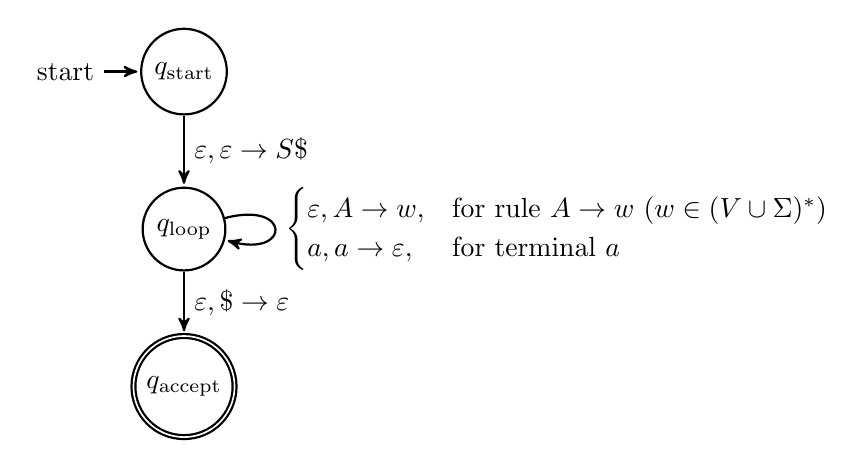
\begin{tikzpicture}[->,>=stealth',shorten >=1pt,auto,node distance=2cm,
			thick,base node/.style={circle,draw,minimum size=16pt}, real node/.style={double,circle,draw,minimum size=35pt}]

			\node[initial, state] (1) {$q_{\text{start}}$};
			\node[state] (2) [below of=1] {$q_{\text{loop}}$};
			\node[state, accepting] [below of=2] (3) {$q_{\text{accept}}$};

			\path[]
			(1) edge node {$\varepsilon, \varepsilon \to S\$$ } (2)
			(2) edge node {$\varepsilon, \$ \to \varepsilon$ } (3)
			(2) edge [loop right] node {$\begin{cases}\varepsilon, A \to w, & \text{for rule } A \to w \ (w \in (V \cup \Sigma)^*)\\ a, a \to \varepsilon, & \text{for terminal }a\end{cases}$} (2);
			
		\end{tikzpicture}
	\end{center}

	“$\Leftarrow$”: 需要根据 PDA 来构造 CFG. 不妨假设\footnote{需要简短地说明转化的可行性. 前两条只需要添加额外的结束状态和转移函数即可, 第三条需要在所有 both 和 neither 的转移中间插入中间状态.}该 PDA 有如下特性:\num{i}只有一个接受态$q_{\text{accept}}$, \num{ii}会在接受前清空栈, \num{iii}每次转移都会要么 push 要么 pop, 没有 both 和 neither 的情况. 构造变量$A_{pq}$表示所有能够使 PDA 从“状态$p$且栈空”转移到“状态$q$且栈空”的串组成的语言, 其中$A_{q_0q_{\text{accept}}}$是该 CFG 的起始变量. 按如下方式构造 CFG 的规则集合:
	\begin{itemize}
		\item 对于任意$p, q, r, s \in Q, u \in \Gamma, a, b \in \Sigma_{\varepsilon}$, 如果$(r, u) \in \delta(p, a, \varepsilon), (q, \varepsilon) \in \delta(s, b, u)$, 就添加规则$A_{pq} \to a A_{rs} b$, 
		\item 对于任意$p, q, r \in Q$, 添加规则$A_{pq} \to A_{pr}A_{rq}$, 
		\item 对于任意$p \in Q$, 添加规则$A_{pp} \to \varepsilon$. 
	\end{itemize}

	构造思路来源于考虑压栈弹栈的括号序列, 该序列要么被一个大括号包裹(第一种), 要么由两个括号序列组成(第二种). 可以归纳证明 $A_{pq}$ 的构造方式与其含义的等价性. 
\end{proof}

\subsection{Pumping Lemma}

\begin{theorem}[Pumping Lemma for CFL]
	如果$A$是上下文无关语言, 那么存在一个数$p$(称为\obj{pumping length}), 使得对于任意$A$中长度至少为$p$的字符串$s$, $s$都可以分成五部分$s = uvxyz$满足
	\begin{itemize}
		\item for each $i \ge 0, uv^ixy^iz \in A$,
		\item $|vy| > 0$,
		\item $|vxy| \le p$.
	\end{itemize}
\end{theorem}
\begin{proof}
	设$b$为规则中的最大“度数”, 即替换字符串的最大长度. 如果 parse tree 的树高是$h$(根的深度是 $0$), 那么生成的字符串长度至多为$b^h$. 

	取 pumping length $p$ 为$b^{|V|+1}$. 长度至少为$p$的串对应的 parse tree 树高至少为$|V| + 1$, 故存在一条“直链”上有至少$|V| + 1$个变量, 根据\obj{鸽巢原理}, 存在一个变量出现至少两次, 记为$R$, 那么对于$R$就可以无限复制或者把两次出现压缩成一次(如图). 

	为了满足第二个条件, 我们要求 parse tree 必须是"最简"的, 因为只有冗余的替换方式才会导致两次 $R$ 的出现之间没有任何字符实际生成.

	为了满足第三个条件, 取$R$为满足条件的“深度最大”的, 即两个$R$都出现在最底下$|V| + 1$层. 此时$|vxy|$对应上面的$R$的子树大小, 受深度限制不超过$b^{|V| + 1} = p$. 
	\begin{center}
		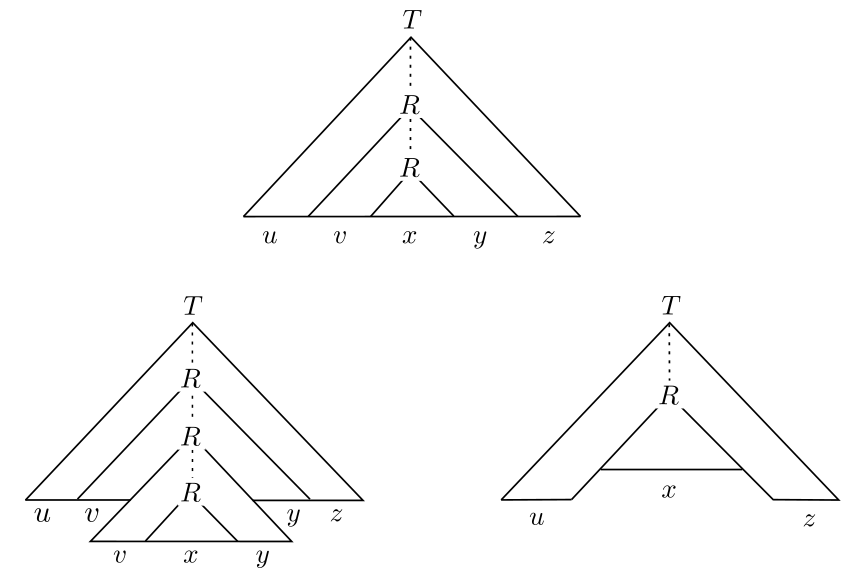
\includegraphics[scale=0.3]{pic/pumping_for_CFL.png}		
	\end{center}
\end{proof}
\begin{example}
	$B = \{a^nb^nc^n | n \ge 0\}$不是上下文无关语言.
\end{example}
\begin{proof}
	假设 B 是正则语言, 那么就存在 pumping length $p$. 考虑串 $a^pb^pc^p$, 注意到 $|vxy| \le p$ 故不可能含有超过两种字符, 那么在重复时就不可能保证三种字符出现次数仍然相同, 从而 $B$ 不是上下文无关语言.
\end{proof}
\begin{example}
	$C = \{a^ib^jc^k | 0 \le i \le j \le k\}$ 不是上下文无关语言.
\end{example}
\begin{proof}
	考虑串 $a^{p}b^{p}b^{p}$, 注意 $v, y$ 分别只能包含一种字符, 否则就会出现顺序错乱. 无论分别包含什么字符, 考虑 pumping up 或者 pumping down, 总可以使得生成的新字符串不属于 $C$, 从而 $C$ 不是上下文无关语言.
\end{proof}
\begin{example}
	$D = \{ww | w \in \{0, 1\}^*\}$ 不是上下文无关语言. 
\end{example}
\begin{proof}
	考虑 $s = 0^p1^p0^p1^p$. 

	首先指出 $vxy$ 必须跨域 $s$ 的中点. 假设 $vxy$ 只出现在 $s$ 的左半边, 那么 $uv^2xy^2z$ 中, 中点右侧的字符一定是 $1$(因为 $|vy| \le p$, 只会把 $\frac{|vy|}{2} \le \frac p2$ 个 $1$ 推到右半边), 而起始字符是 $0$ 说明该串不是 $ww$ 形式的. 

	但如果 $vxy$ 跨越 $s$ 的中点, 那么就一定跟前 $p$ 个 $0$ 与后 $p$ 个 $1$ 无交, 因此 $uxz$ 就会形如 $0^p1^i0^j1^p$, 其中 $i, j < p$, 这显然不属于 $D$.
\end{proof}

\newpage
\section{图灵机}

图灵机是有限自动机的进一步加强(也严格强于下推自动机), 在状态集的基础上额外添加了外部存储设备——“纸带”. 一条纸带是一列无限长的存储单元(称为“格子”), 其中每个格子上只能存储有限的信息, 在单步计算中也只能读取/写入一个格子, 读取/写入的格子位置(称为“纸带头”)在相邻两步计算间也至多移动一格. 

通俗地来讲, 一台拥有 $k$ 条纸带的图灵机在一步计算中, 会首先查询其状态并分别在 $k$ 个纸带头位置读取 $k$ 个字符, 然后根据这些信息, 决定变换到什么状态, 将 $k$ 个纸带头处的字符改写成什么, 以及如何移动 $k$ 个纸带头(向左或右移动一格, 或者保持不动). 

\begin{definition}[Deterministic Turing Machine, TM]
	一台 $k$ 条纸带的 (确定性)图灵机是一个七元组 \\ $(Q, \Sigma, \Gamma, \delta, q_0, q_{\text{accept}}, q_{\text{reject}})$, 其中
	\begin{itemize}
		\item $Q$ 是状态集.
		\item $\Sigma$ 是不包含空格符$\Box$的输入字符集, $\Gamma$ 是纸带字符集. $\Sigma \subseteq \Gamma$.
		\item $\delta: Q \times \Gamma^k \to Q \times \Gamma^k \times \{\text{L(eft), S(tay), R(ight)}\}^k$ 是转移函数.
		\item $q_0, q_{\text{accept}}, q_{\text{reject}} \in Q$ 分别是起始态, 接受态和拒接态.
	\end{itemize}

	初始时, 第一条纸带的第一个格子上标有 $\triangleright$ 字符, 表示输入串的开始, 随后紧接着是输入串 $w \in \Sigma^*$. 除了这 $|w| + 1$ 个格子外, 所有纸带的所有格子都被初始化为空格符 $\Box$.

	一旦图灵机运行到 $q_{\text{accept}}$ 或者 $q_{\text{reject}}$ 状态时, 它就会\obj{停机}. 因此可以把一台图灵机看成一个 $\Sigma^* \to \{0, 1\}$ 的函数. 一般地, 对于图灵机 $M$ 和字符串 $x \in \Sigma^*$, 我们有 $M(x) \in \{0, 1\}$, 其中 $M(x) = 1$ 当且仅当对于输入 $x$, $M$ 会运行到$q_{\text{accept}}$, $M(x) = 0$ 当且仅当对于输入 $x$, $M$ 会运行到 $q_{\text{reject}}$ \obj{或者不停机}.

	\iffalse
	图灵机的一个 \obj{configuration} 包含其状态, 所有纸带上的字符, 以及所有纸带头的位置. 称图灵机 $M$ 接受字符串 $w$, 如果存在一个 configuration 序列 $C_0, C_1, \cdots, C_t$ 满足 \num{i} $C_0$ 是起始 configuration, i.e.  \num{ii} 每个 $C_i$ 都在一步内跳转到 $C_{i+1}$, \num{iii} $C_t$ 是接受 configuration.
	\fi

	对于图灵机 $M$, 记 $L(M) = \{x \in \{0, 1\}^* | M(x) = 1\}$ 为 $M$ 所\obj{识别}的语言.
\end{definition}
\begin{remark}
	图灵机还存在另一种设定: 并没有 $q_{\text{accept}}, q_{\text{reject}}$ 两个特殊状态, 取而代之的是单一的停机状态 $q_{\text{halt}}$, 同时最后一条纸带被用作“输出纸带”. 图灵机运行到 $q_{\text{halt}}$ 时停机, 此时输出纸带上的内容就是该图灵机的输出. 

	这种设定下的图灵机可以看作一个 $\Sigma^* \to \Sigma^*$ 的函数, 但不难验证其计算能力与原本设定下的是相同的. 之后为了省事可能会混淆使用两种设定, 不妨碍理解就好.
\end{remark}
\begin{definition}[图灵可识别与图灵可判定]
	称一个语言是\obj{图灵可识别(Turing-recognizable)}的, 如果存在一台图灵机可以识别它(i.e. 接受其中的每一个字符串). 称一台图灵机是一个 \obj{decider}, 如果它对于任何输入都不会无限循环. 称一个语言是\obj{图灵可判定(Turing-decidable)}的, 如果存在一台 decider 可以识别它.
\end{definition}
\begin{definition}[函数的计算, 运行时间]
	考虑函数 $f: \{0,  1\}^* \to \{0, 1\}^*$ 以及 $T: \mathbb{N} \to \mathbb{N}$, 令 $M$ 为一图灵机. 我们称 $M$ 计算了函数 $f$, 如果对于任意 $x \in \{0, 1\}^*$, 只要 $M$ 被初始化为输入$x$, 它就能在输出纸带上写下 $f(x)$ 并停机. 称 $M$ 在 $T(n)$ 的时间内计算了 $f$, 如果它计算每个 $x$ 都可以在 $T(|x|)$ 步内停机.
\end{definition}
\begin{definition}[Time-constructible functions]
	称一个函数 $T: \mathbb N \to \mathbb N$ 是 time-constructible的, 如果 $T(n) \ge n$ 且存在运行时间为 $T(n)$ 的计算函数 $x \to \rep{T(|x|)}$ 的图灵机 $M$, 其中 $\rep{x}$ 表示 $x$ 的 binary representation.
\end{definition}
\begin{example}
	$A = \{w \# w | w \in \{0, 1\}^*\}$ 可以被(单纸带)图灵机识别.
\end{example}
\begin{proof}
	给待匹配的两个位置打上标记, 每次前后移动找标记, 用状态记录已经看过的字符, 若比较失败则直接 reject, 否则向后移动标记继续比较直到全部比完. 以上的描述的图灵机的运行时间是 $T(n) = O(n^2)$ 的.
\end{proof}
\begin{example}
	$B = \{ww | w \in \{0, 1\}^*\}$ 可以被双纸带图灵机识别.
\end{example}
\begin{proof}
	\textit{没有 \# 记号, 无法方便地找到中间位置.} 可以在二号纸带上把输入复制一遍, 然后二号纸带头移动到中间(一号纸带头走一步, 二号纸带头走两步), 顺序比较即可. 运行时间是 $O(n)$.
\end{proof}

图灵机由字符集大小, 纸带数量等的不同, 产生了许多不同的变种. 它们在计算能力上会有所不同吗?

\begin{proposition}[小字符集模拟大字符集]
	对于任意$f: \{0, 1\}^* \to \{0, 1\}$以及time-constructible function $T: \mathbb{N} \to \mathbb{N}$, 如果$f$可以被图灵机$M$以$T(n)$时间计算, 那么它也可以被一台字符集为$\{0, 1, \Box, \triangleright\}$的图灵机$\tilde{M}$以$O(T(n)\log |\Gamma|)$的时间计算. 
\end{proposition}
\begin{proof}
	任意 $\Gamma$ 中的字符都可以用 $\log |\Gamma|$ 个比特表示. 每步转移时先用 $\log |\Gamma|$ 步读出纸带上一个字符的 encoding 并存入状态, 再根据转移函数进行移动, 最后用 $\log |\Gamma|$ 步写下新字符的 encoding 表示.
\end{proof}
\begin{proposition}[单纸带模拟多纸带]
	对于任意$f: \{0, 1\}^* \to \{0, 1\}$以及time-constructible function $T: \mathbb{N} \to \mathbb{N}$, 如果$f$可以被有$k$条纸带的图灵机$M$以$T(n)$时间计算, 那么它也可以被一台单纸带图灵机$\tilde{M}$以$O(kT^2(n))$的时间计算. 单纸带指的是只有一条可读可写的纸带, 它同时扮演了输入、工作和输出纸带的角色. 
\end{proposition}
\begin{proof}
	把单条纸带上的位置按照模 $k$ 余数分配给 $k$ 条纸带, 对每种字符 $a$ 新建字符 $\hat a$ 表示所在纸带的纸带头指向这个字符. 注意到运行时间为 $T(n)$ 的图灵机, 对于长度为 $n$ 的输入, 最多只会用到前 $T(n)$ 个位置, 所以每步转移时花费 $O(kT(n))$ 的代价搜索每个纸带头的位置即可\footnote{可以考虑在已使用部分的“最远处”打上标记并维护, 这样每次搜索的代价就不超过当前写入过的格子数量}, 运行时间为 $O(kT^2(n))$.
\end{proof}
\begin{remark}[健忘的图灵机, oblivious Turing Machine]
	纸带头的移动只与输入长度有关, 而与输入的具体内容无关, 即对于任意$x \in \{0, 1\}^*$以及$i \in \mathbb N$, $M$在输入 $x$ 并执行到第$i$步时, 所有纸带头的位置是关于$|x|$和$i$的函数. 可以证明健忘的图灵机可以以平方的overhead模拟一台标准图灵机. 
	\label{oblivious}
\end{remark}
\begin{proposition}[单向图灵机模拟双向图灵机]
	对于任意$f: \{0, 1\}^* \to \{0, 1\}$以及time-constructible function $T: \mathbb{N} \to \mathbb{N}$, 如果$f$可以被双向图灵机(纸带的两个方向都有无限长)$M$以$T(n)$时间计算, 那么它也可以被一台单向图灵机$\tilde{M}$以$O(T(n))$的时间计算. 
\end{proposition}
\begin{thesis}[Church-Turing Thesis]
	任何物理上可实现的计算设备都可以被图灵机实现. 
\end{thesis}
\begin{theorem}[通用图灵机存在]
	存在图灵机$\mathcal U$使得对于任意$x, \alpha \in \{0, 1\}^*$, $\mathcal U(\langle x, \alpha \rangle ) = M_{\alpha}(x)$, 其中$M_{\alpha}$为被$\alpha$表示的图灵机. 进一步地, 如果$M_{\alpha}$对于$x$在$T$步内停机, 则$\mathcal U(\langle x, \alpha \rangle )$可以在$CT\log T$步内停机, 其中$C$是一个仅依赖于$M_{\alpha}$的字符集大小、纸袋条数、状态数的常数. 
\end{theorem}
\begin{proof}
	构造 $\mathcal U$ 为一台五纸带图灵机, 五条纸带分别为
	\begin{itemize}
		\item Input, 被模拟图灵机 $M$ 的输入.
		\item Description of $M$, 主要为了记录转移函数 $\delta$ 以便查询.
		\item Simulation of $M$, 记录纸带信息. 这里需要用单纸带来模拟 $M$, 因而会产生平方的 overhead.
		\item Current state of $M$, 这部分不能简单地存在 $\mathcal U$ 的状态里, 因为对于 $\mathcal U$ 来说, $M$ 的状态集大小并不是常数.
		\item Output, $M$ 的输出.
	\end{itemize}

	注意每步模拟的过程中, 读取 $M$ 所在状态, 读取转移函数都是关于 $n$ 常数时间的.

	可以设计一种基于势能分析的算法, 把单纸带模拟多纸带的 overhead 降到 $O(n \log n)$, 从而使通用图灵机模拟的复杂度优化到 $O(T \log T)$.
\end{proof}

\newpage
\section{不可判定语言}
\begin{definition}[可识别/判定语言, recognizable/decidable Language]
	可识别语言就是能够被一台图灵机识别的语言. 可判定语言就是能够被一台 decider 识别的语言.
\end{definition}
\begin{theorem}
	存在不可识别语言.
	\label{unrecognize_exists}
\end{theorem}
\begin{proof}
	只需要考虑“语言”与“可识别语言”的基数. 前者的基数是 $2^{\aleph_0}$, 后者的基数不超过图灵机的基数(因为存在可识别语言到图灵机的单射), 而图灵机可以被有限长的字符串描述, 因此是可数的.
\end{proof}
\begin{definition}[可计算函数(Computable Function)]
	可计算函数就是可以被一台图灵机计算的函数. 特别的, 考虑函数 $f: \{0, 1\}^* \to \{0, 1\}$, 则 $f$ 是可计算函数当且仅当 $L = \{x \in \{0, 1\}^*| f(x) = 1\}$ 是可判定语言.
\end{definition}
\begin{theorem}
	存在不可计算函数/存在不可判定语言. (证明中的构造是重要的. 结论本身相比\cref{unrecognize_exists} 是平凡的.)
\end{theorem}
\begin{proof}
	我们认为存在一个映射$\alpha \to M_{\alpha}$可以把任意字符串映到一台图灵机(以某种既定格式编码, 再把非法格式的串映到某台特定的图灵机即可). 考虑函数 $\text{UC}(\alpha) = 1 - M_{\alpha}(\alpha)$, 我们指出 $\text{UC}$ 是不可计算函数.

	假设 $\text{UC}$ 可计算, 考虑计算 $\text{UC}$ 的图灵机 $M$. 考虑 $\text{UC}(\rep{M})$, 由于 $M$ 计算了 $\text{UC}$, 我们知道 $\text{UC}(\rep{M}) = M(\rep M)$, 但根据 $\text{UC}$ 的定义, 又有 $\text{UC}(\rep M) = 1 - M(\rep M)$, 产生了矛盾.
\end{proof}
\begin{example}[停机问题不可判定]
	$\textsf{HALT} = \{\langle \rep M, \alpha \rangle | M \text{ halts on } \alpha\}$ 是不可判定语言.
\end{example}
\begin{proof}
	假设存在 $M_{\textsf{HALT}}$ 可以判定 $\textsf{HALT}$.
	
	利用 $M_{\textsf{HALT}}$ 可以构造判定语言 $L = \{\alpha | \text{UC}(\alpha) = 1\}$ 的 decider: 计算 $M_{\textsf{HALT}}(\langle \alpha, \alpha \rangle)$, 如果得到 $0$ (说明 $M_{\alpha}$ 对 $\alpha$ 不停机) 则直接输出 $1$, 否则输出$M_{\alpha}(\alpha)$ 的结果. 这与 $\text{UC}$ 不可计算相矛盾. 因此 \textsf{HALT} 不可判定.
\end{proof}
\begin{example}[接受问题不可判定]
	$\textsf{AC} = \{\langle \rep M, \alpha \rangle | M \text{ accepts } \alpha\}$ 是不可判定语言.	
\end{example}
\begin{proof}
	利用 $M_{\textsf{AC}}$ 可以直接构造 $M_{\text{UC}}$: 只要把 $M_{\textsf{AC}}(\langle \alpha, \alpha \rangle)$ 的输出取反即可.
\end{proof}
\begin{definition}[映射规约, Mapping Reduction]
	称语言 $A$ 可映射规约到(is mapping reducible to) 语言 $B$, 如果存在可计算函数 $f: \Sigma^* \to \Sigma^*$, 使得 $w \in A$ 当且仅当 $f(w) \in B$, 记作 $A \le_m B$.
\end{definition}
\begin{proposition} 如果 $A \le_m B$, 则
	\begin{itemize}
		\item 如果 $B$ 可判定, 则 $A$ 也可判定.
		\item 如果 $A$ 不可判定, 则 $B$ 也不可判定.
	\end{itemize}
\end{proposition}
\begin{example}
	$\textsf{NAC} = \{\rep M | M \text{ accept nothing}\}$ 是不可判定语言.
\end{example}
\begin{proof}
	考虑构造映射 $f$ 满足 $w \in \overline{\textsf{AC}} \Leftrightarrow f(w) \in \textsf{NAC}$. 令 $f(\langle \rep M, \alpha \rangle) = \rep{M'}$ 其中 $M'$ 不管输入直接运行 $M(\alpha)$. $f$ 显然是可计算的, 故 $\overline{\textsf{AC}} \le_m \textsf{NAC}$, 而可判定语言关于补集的封闭性导致 $\overline{\textsf{AC}}$ 是不可判定语言, 从而 $\textsf{NAC}$ 是不可判定语言.
\end{proof}
\begin{example}
	$\textsf{EQU} = \{\langle \rep{M_1}, \rep{M_2} \rangle | L(M_1) = L(M_2)\}$ 是不可判定语言.
\end{example}
\begin{proof}
	考虑构造映射 $g$. 取 $g(\rep{M}) = \langle \rep{M}, \rep{M'}\rangle$ 其中 $M'$ 是拒绝一切输入的图灵机. 于是 $\rep{M} \in \textsf{NAC} \Leftrightarrow \langle \rep{M}, \rep{M'}\rangle \in \textsf{EQU}$, $\textsf{NAC} \le_m \textsf{EQU}$, 从而 \textsf{EQU} 是不可判定语言.
\end{proof}
\begin{theorem}
	语言 $A$ 可判定当且仅当 $A$ 与 $\overline{A}$ 均可识别.
\end{theorem}
\begin{proof}
	$\Rightarrow$: 显然. $\Leftarrow$: 记 $A$ 可被 $M_1$ 识别, $\overline A$ 可被 $M_2$ 识别, 考虑\obj{并行}运行 $M_1$ 和 $M_2$, 总有一个会给出结果. 
\end{proof}
\begin{corollary}
	\textsf{HALT} 和 \textsf{AC} 都是不可判定的可识别语言. 这说明 $\overline{\textsf{HALT}}$ 和 $\overline{\textsf{AC}}$ 都是不可识别语言.
\end{corollary}

\newpage
\section{时间复杂性, \P 与 \NP}
\subsection{\P \ verses \NP}
\begin{definition}[\DTIME 与 \P]
	对于函数$T: \mathbb N \to \mathbb N$, 称语言$L \in \DTIME(T(n))$, 如果存在常数$c > 0$和一台运行时间为$c \cdot T(n)$的 decider 可以识别$L$. 定义 $\P = \bigcup_{c \ge 0}\DTIME(n^c)$. 
\end{definition}
\begin{proposition}
	$\P$ 在多项式次集合操作下是封闭的.
\end{proposition}
\begin{example}
	$\textsf{PATH} = \{ \langle G, s, t\rangle : G \textrm{ is a direct graph in which there is a path from }s \textrm{ to } t\} \in \P.$
\end{example}
\begin{theorem}[Time Hierarchy Theorem]
	$f, g$是满足$f(n) \log f(n) = o(g(n))$的time constructible的函数, 则
	$$\DTIME(f(n)) \subsetneq \DTIME(g(n))$$
	\label{time_hierarchy_thm}
\end{theorem}
\begin{proof}
	考虑这样的图灵机$D$:对于$x \in \{0, 1\}^*$, 用通用图灵机$\mathcal{U}$模拟$M_x(x)$运行至多$g(|x|)$步(是$\mathcal U$的$g(|x|)$步而不是$M_x$的$g(|x|)$步), 如果$\mathcal{U}$在$g(|x|)$步数内输出了$b \in \{0, 1\}$, 则$D$输出$1-b$, 否则$D$输出$0$. 

	根据定义, $D$对于任何输入$x$都会在$g(|x|)$步内停机, 因此$L(D) \in \DTIME(g(n))$. 我们通过反证法证明$L(D) \notin \DTIME(f(n))$. 先叙述否命题: 存在图灵机$M$和常数$c$, 使得对于任意输入$x \in \{0, 1\}^*$, $M$都能在$cf(|x|)$步内输出与$D$相同的结果. 

	对于输入$x$, 用通用图灵机$\mathcal{U}$模拟$M$只需要$c'cf(|x|)\log f(|x|)$步, 其中$c'$是不依赖于$|x|$的一个常数. 由于$f(n) \log f(n) = o(g(n))$, 故存在充分大的$n_0$使得$g(n) > c'cf(n) \log f(n)$对于任意$n \ge n_0$均成立. 令$x' = \rep{M}$ 满足 $|x'| \ge n_0$, 那么
	\begin{itemize}
		\item $D$会输出与$M$相同的结果, 因为这是$M$的定义;
		\item $D$会输出与$M$不同的结果, 因为$c'cf(n)\log f(n) < g(n)$使得$\mathcal U$对$M$的模拟已经结束了, 根据$D$的定义, $D$应该输出相反的结果. 
	\end{itemize}

	产生了矛盾. 因此$\DTIME(f(n)) \subsetneq \DTIME(g(n))$. 
\end{proof}
\begin{definition}[\NP]
	称语言$L \subseteq \{0, 1\}^*$属于\NP, 如果存在一个多项式$p: \mathbb N \to \mathbb N$和一个多项式时间图灵机$M$(称为$L$的\obj{verifier})使得对于任意的$x \in \{0, 1\}^*$, 都有
	$$x \in L \Leftrightarrow \exists u \in \{0, 1\}^{p(|x|)}, M(x, u) = 1$$
	如果$x \in L$与$u \in \{0, 1\}^{p(|x|)}$满足$M(x, u) = 1$, 则称$u$是$x$的一个\obj{certificate}. 
\end{definition}
\begin{proposition}
	定义$\EXP = \bigcup_{c \ge 0} \DTIME(2^{n^c})$, 则$\P \subseteq \NP \subseteq \EXP$. 
\end{proposition}
\begin{remark}
	根据 Time Hierarchy Theorem 我们知道 $\P \subsetneq \EXP$, 因此 $\P \subsetneq \NP$ 与 $\NP \subsetneq \EXP$ 至少一者为真.
\end{remark}
\begin{definition}[非确定图灵机与\NTIME]
	非确定图灵机(Nondeterministic Turing Machine, NDTM)是有两个转移函数$\delta_0, \delta_1$和一个特定状态$q_{\text{accept}}$的图灵机$M$, 每步转移时, 可以任意选择遵从某一个转移函数. 对于输入$x$, 称$M(x) = 1$当且仅当存在一个选择序列可以使$M$到达$q_{\text{accept}}$状态, 否则——任意选择序列都无法在停机前到达$q_{\text{accept}}$——就认为$M(x) = 0$. 称$M$的运行时间为$T(n)$, 如果对于任意输入$x \in \{0, 1\}^*$以及任意的选择序列, $M$都会在$T(|x|)$步内到达$q_{\text{accept}}$或者$q_{\text{halt}}$. 

	对于$T: \mathbb N \to \mathbb N$和语言$L \subseteq \{0, 1\}^*$, 称$L \in \NTIME(T(n))$, 如果存在常数$c > 0$和一个运行时间为$c \cdot T(n)$的非确定图灵机$M$, 满足对于任意的$x \in \{0, 1\}^*$, $x \in L \Leftrightarrow M(x) = 1$. 
\end{definition}
\begin{theorem}
	$\NP = \bigcup_{c \ge 0} \NTIME(n^c)$. 
\end{theorem}
\begin{proof}
	非确定图灵机的选择序列可以看作$x$的一个 certificate, 反之亦然. 
\end{proof}

\subsection{\NP 完全性}
\begin{definition}[多项式时间规约, \NP-hard 与 \NP-complete]
	称语言$L \subseteq \{0, 1\}^*$可\obj{多项式时间(Karp)规约}到语言$L' \subseteq \{0, 1\}^*$(记作$L \le_p L'$), 如果存在一个多项式时间可计算函数$f: \{0, 1\}^* \to \{0, 1\}^*$使得对于任意$x \in \{0, 1\}^*$, $x \in L \Leftrightarrow f(x) \in L'$. 

	称$L' \in $ \NP-hard, 如果对于任意$L \in \NP$, $L \le_p L'$. \NP-complete $=$ \NP\ $\cap$ \NP-hard.  
\end{definition}
\begin{theorem}[$\le_p$的传递性]
	\begin{itemize}
		\item 若$L \le_p L'$且$L' \le_p L''$, 则$L \le_p L''$. 
		\item 如果$L \in $ \NP-hard, 则$L \in \P \Rightarrow \P = \NP$. 
		\item 如果$L \in $ \NP-complete, 则$L \in \P \Leftrightarrow \P = \NP$. 
	\end{itemize}
\end{theorem}
\begin{theorem}[Cook-Levin Theorem]
	$\textsf{SAT}, \textsf{3SAT} \in $ \NP-complete. 

	其中 $\textsf{SAT} = \{\varphi \in \text{CNF} | \varphi \text{ is satisfiable}\}, \textsf{3SAT} = \{\varphi \in 3\text{CNF} | \varphi \text{ is satisfiable}\}$. CNF(Conjunctive Normal Form, 合取范式)是一种形如 $\bigwedge_i\left(\bigvee_j v_{i_j}\right)$ 的特殊的 boolean formula, 其中每个 $v_{i_j}$ 都是某个变量或者其否定. 3CNF 是每个 $\bigvee_j v_{i_j}$ (称为\obj{从句(clause)})中都只含有不超过 $3$ 项的 CNF.
\end{theorem}
\begin{proof}
	$\textsf{SAT}, \textsf{3SAT} \in \NP$ 是平凡的. 先考虑证明 $\textsf{SAT} \in \NP$-hard, 即 $\forall L \in \NP, L \le_p \textsf{SAT}$. 回顾两者定义
	\begin{center}		
		\begin{tabular}{cccc}
			$x \in L$ & $\Leftrightarrow$ & $\exists$ certificate $u$ & s.t. $M(x, u) = 1$\\
			$\varphi_x \in \textsf{SAT}$ & $\Leftrightarrow$ & $\exists$ assignment $u$ & s.t. $\varphi_x(u) = \text{True}$\\
		\end{tabular}
	\end{center}
	因此考虑根据 $M, x$ 来构造\obj{多项式规模的} $\varphi_x$, 满足 $M(x, u) = 1 \Leftrightarrow \varphi_x(u) = \text{True}$. 
	
	不妨假设 $M$ 是 \num{i} 双纸带且第一条纸带只读 \num{ii} oblivious 的(参见\cref{oblivious}), 那么在$M$运行到第 $i$ 步时, 其两个纸带头所指向的字符, 当前状态所组成的三元组 $z_i \in \Gamma \times \Gamma \times Q$ (称为 $M$ 运行到第 $i$ 步时的 \obj{snapshot})将由后三者唯一决定: $z_{i-1}, z_{\text{prev}(i)}$ 和 $(x \circ u)_{\text{inputpos}(i)}$, 其中 $\text{prev}(i)$ 表示上一次工作纸带纸带头位置与第$i$步相同的时刻, $\text{inputpos}(i)$ 表示第 $i$ 步时输入纸带的纸带头位置.

	根据 $M$ 的转移函数 $\delta$, 可以构造出 $F: \{0, 1\}^{2c+1} \to \{0, 1\}^c$ 满足 $z_i = F(z_{i-1}, z_{\text{prev}(i)}, (x \circ u)_{\text{inputpos}(i)})$, 其中 $c$ 是表示一个 snapshot 所需的比特数. 

	可以构造一个有 $n + p(n) + cT(n)$ 个变量的 CNF $\varphi_x$, 其中 $p, T$ 是 $M$ 的参数(分别是verifier 长度与运行时间关于 $n$ 的函数). 把这些变量分别记为 $y$ 以及 $z_1, \cdots, z_{T(n)}$, 它是下述这些条件的 AND:
	\begin{enumerate}
		\item $y$ 的前 $n$ 位和 $x$ 相同.
		\item $z_1$ 表示初始状态 $(\triangleright, \Box, q_{\text{start}})$.
		\item $z_i = F(z_{i-1}, z_{\text{prev}(i)}, y_{\text{inputpos}(i)}) \ (\forall i \in \{2, \cdots, T(n)\})$.
		\item $z_{T(n)}$ 表示到达 $q_{\text{halt}}$ 的终止状态.
	\end{enumerate}

	这些条件用 CNF 表示出来, 其长度是 $d(n + T(n))$, 其中 $d$ 是与 $n$ 无关的常数. 从而我们实现了多项式时间规约, 完成了 $L \le_p \textsf{SAT}$ 的证明.

	然后考虑证明 $\textsf{SAT} \le_p \textsf{3SAT}$. 只需要注意到
	$$\bigvee_{i=1}^{k}u_i \cong \left(z \vee \bigvee_{i=1}^{k-2}u_i\right) \wedge (\overline{z} \vee u_{k-1} \vee u_{k})$$
	说明任意 CNF 都可以多项式时间规约到 3CNF. 所以 $\textsf{SAT} \le_p \textsf{3SAT}$.
\end{proof}
\subsection{常见 \NP-complete 问题的规约}
\begin{example}[独立集]
	$\textsf{INDSET} = \{\langle G, k \rangle | G \text{ has an independent set of size } k\} \in \NP$-complete.
\end{example}
\begin{proof}
	显然 $\textsf{INDSET} \in \NP$. 考虑通过 $\textsf{3SAT} \le_p \textsf{INDSET}$ 来证明 $\textsf{INDSET} \in \NP$-hard.

	对于一个有 $m$ 个 clause 的 3CNF $\varphi$, 对每个有 $l$ 项的 clause 建不超过 $2^l$ 个点, 表示能使这个 clause 为 True 的部分变量赋值(互不相同). 在所有会产生冲突的点对间连边, 得到一张不超过 $7m$ 个点的图. 不难验证这张图存在大小为 $m$ 的独立集当且仅当 $\varphi$ 可满足.
\end{proof}
\begin{example}[点覆盖]
	$\textsf{Vertex-Cover} = \{\langle G, k \rangle | G \text{ has a subset of } k \text{ vertices that covers all edges}\} \in \NP$-complete.
\end{example}
\begin{proof}
	独立集很容易规约到点覆盖, 懂的都懂.
\end{proof}
\begin{example}[01整数规划]
	给出一列有理系数线性不等式, 判断是否存在一组 $\{0, 1\}$ 赋值满足所有不等式. 把可满足的不等式组的集合记作 $\textsf{01IPROG}$. $\textsf{01IPROG} \in \NP$-complete.
\end{example}
\begin{proof}
	考虑证明 $\textsf{SAT} \le_p \textsf{01IPROG}$. 只需要对每个 clause 构造一个不等式即可.
	$$u_1 \vee \cdots \vee u_n \vee \overline{u_{n+1}} \vee \cdots \vee \overline{u_{n+m}} \Rightarrow \sum_{i=1}^{n}u_i + m - \sum_{i=1}^{m}u_{n+i} \ge 1$$
\end{proof}
\begin{remark}
	如果把变量取值限制从 $\{0, 1\}$ 改为全体有理数, 问题就变成了线性规划, 从而 $\in \P$.
\end{remark}
\begin{example}
	$\textsf{DSAT} = \{\varphi \in \text{DNF} | \varphi \text{ is satisfiable}\} \in \P$. 只要线性地检查一下有没有某个 clause 都满足就行了.
\end{example}
\begin{example}[有向图哈密顿路径]
	$\textsf{dHAMPATH} = \{\rep{G} | G \text{ is directed and has a Hamiltonian path}\} \in \NP$-complete.
\end{example}
\begin{proof}
	考虑证明 $\textsf{SAT} \le_p \textsf{dHAMPATH}$. 对于一个有 $n$ 个变量和 $m$ 个 clause 的 CNF $\varphi$:
	\begin{itemize}
		\item 对每个变量建 $2m + 1$ 个点, 第 $i$ 个变量对应的点记作 $a_{i, 1}, \cdots, a_{i, 2m+1}$. 对每个 clause 建一个点, 第 $i$ 个 clause 对应的点记作 $b_i$. 再建立额外源汇 $v_{\text{start}}, v_{\text{end}}$, 总共是 $(2m+1)n + m + 2$ 个点.
		\item 对于每个 $i \in [1, n]$, $a_{i, 1}, \cdots, a_{i, 2m+1}$ 首尾相接连成一个 $2m+1$ 大小的\obj{双向}环.
		\item $v_{\text{start}}$ 向 $\{a_{1, 1}, a_{1, 2m+1}\}$ 连边, $\{a_{i, 1}, a_{i, 2m+1}\}$ 向 $\{a_{i+1, 1}, a_{i+1, 2m+1}\}$ 连边, $\{a_{n, 1}, a_{n, 2m+1}\}$ 向 $v_{\text{end}}$ 连边, 均为单向.
		\item 如果 $u_i$ 出现在了第 $j$ 个从句中, 连边$a_{i, j} \to b_j \to a_{i, j+1}$. 如果 $\overline{u_i}$ 出现在了第 $j$ 个从句中, 连边$a_{i, j+1} \to b_j \to a_{i, j}$.
	\end{itemize}

	对于每个双向环, 它可以也应该被顺时针或者逆时针地单向遍历, 即要么首先访问 $a_{i, 1}$ 然后从小到大走到 $a_{i, 2m+1}$, 要么首先访问 $a_{i, 2m+1}$ 然后从大到小走到 $a_{i, 1}$. 顺/逆时针的遍历方向对应着相应变量的 $0/1$ 取值, 当取值符合期望时, 遍历该变量对应的环时可以顺带覆盖掉一些 $b_j$.

	可以证明 $\varphi \in \textsf{SAT}$ 当且仅当上述构造出的图存在 $v_{\text{start}}$ 到 $v_{\text{end}}$ 的哈密顿路径.
\end{proof}
\begin{example}[有向图哈密顿回路]
	$\textsf{dHAMCYCLE} = \{\rep{G} | G \text{ is directed and has a Hamiltonian cycle}\} \in \NP$-complete.
\end{example}
\begin{proof}
	考虑证明 $\textsf{dHAMPATH} \le_p \textsf{dHAMCYCLE}$. 对于图 $G$, 添加额外源汇 $s, t$, $s$ 向所有点连边, 所有点向$t$连边, $t$ 向 $s$ 连边, 得到图 $G'$. $G$ 存在哈密顿路径当且仅当$G'$存在哈密顿回路.
\end{proof}
\begin{example}[无向图哈密顿路径]
	$\textsf{uHAMPATH} = \{\rep{G} | G \text{ is undirected and has a Hamiltonian path}\} \in \NP$-complete.
\end{example}
\begin{proof}
	考虑证明 $\textsf{dHAMPATH} \le_p \textsf{uHAMPATH}$. 

	对于有向图 $G$, 添加额外源汇$s, t$(要连边)后把每个点拆成三个点: 入点, 中间点, 出点, 适当连边得到无向图 $G'$. $G$存在哈密顿路径 $\Rightarrow G'$ 存在哈密顿路径是显然的, 而如果 $G'$ 存在哈密顿路径, 则任意一个入点/出点都会与其中间点相邻, 因为否则会导致中间点不得不成为路径的起止点, 而显然 $s$ 的入点与 $t$ 的出点是必须作为起止点的(度数是 $1$). 于是$G'$的哈密顿路径不会破坏 $G$ 的有向图结构, 从而可以构造出 $G$ 的哈密顿路径.	
\end{proof}
\begin{example}[无向图哈密顿回路]
	$\textsf{uHAMCYCLE} = \{\rep{G} | G \text{ is undirected and has a Hamiltonian cycle}\} \in \NP$-complete.
\end{example}
\begin{proof}
	考虑证明 $\textsf{dHAMCYCLE} \le_p \textsf{uHAMCYCLE}$.

	对于有向图 $G$, 直接把每个点拆成三个点: 入点, 中间点, 出点, 适当连边得到无向图 $G'$. $G$存在哈密顿回路 $\Rightarrow G'$ 存在哈密顿回路是显然的, 而如果 $G'$ 存在哈密顿回路, 则这条回路必然是“入-中间-出-入-中间-出”循环的, 因此也可以构造出 $G$ 的哈密顿回路.
\end{proof}
\begin{example}[旅行商问题]
	$\textsf{TSP} = \{\langle G, d_{ij}, k \rangle | G \text{ has a Hamiltonian cycle with distance measured by } d_{ij} \text{ at most }k\} \in \NP$-complete.
\end{example}
\begin{proof}
	考虑证明 $\textsf{dHAMCYCLE} \le_p \textsf{TSP}$. 根据 $G$ 到底有没有这条边把边权设为 $0$ 或者 $1$, $k$取 $0$ 就行.
\end{proof}

\subsection{\coNP, \NP-intermediate 以及更多}
\begin{definition}[\coNP]
	$\coNP = \{L | \overline{L} \in \NP\}$.
\end{definition}
\begin{example}
	$\overline{\textsf{SAT}} \in \coNP$, 但在证明 $\overline{\textsf{SAT}} \in \NP$ 时遇到了困难: 难以高效地验证 $\varphi$ 对所有的 assignment 都为 False.
\end{example}
\begin{definition}[\coNP 的另一种定义]
	称语言$L \subseteq \{0, 1\}^*$属于\coNP, 如果存在一个多项式$p: \mathbb N \to \mathbb N$和一个多项式时间图灵机$M$使得对于任意的$x \in \{0, 1\}^*$, 都有
	$$x \in L \Leftrightarrow \forall u \in \{0, 1\}^{p(|x|)}, M(x, u) = 0$$
\end{definition}
\begin{definition}[\coNP-hard, \coNP-complete]
	称 $L \in \coNP$-hard, 如果任意 $L' \in \coNP$ 都满足 $L' \le_p L.$ 定义 \coNP-complete = $\coNP \cap \coNP$-hard.
\end{definition}
\begin{example}
	$\overline{\textsf{SAT}} \in \coNP$-complete. 这是因为$\forall L \in \coNP$, 我们有 $\overline L \in \NP$. 由 Cook-Levin Thm. 知 $\overline L \le_p \textsf{SAT}$, 于是便有 $L \le_p \overline{\textsf{SAT}}$. ($A \le_p B \Leftrightarrow \overline A \le_p \overline B$.)
\end{example}
\begin{proposition}
	如果 $\P = \NP$, 则 $\NP = \coNP$. 反过来说, 只要证明了 $\NP \neq \coNP$, 就能说明 $\P \neq \NP$.
\end{proposition}
\begin{definition}[\NEXP]
	$\NEXP = \bigcup_{c \ge 0}\NTIME(2^{n^c})$.
\end{definition}
\begin{theorem}
	如果 $\EXP \neq \NEXP$, 则 $\P \neq \NP$.
\end{theorem}
\begin{proof}
	考虑证明逆否命题: 如果 $\P = \NP$, 则 $\EXP = \NEXP$. 使用一种叫做\obj{填充(padding)}的技术: 考虑 $L \in \NTIME(2^{n^c})$, 构造 $L_{\text{pad}} = \{\langle x, 1^{2^{|x|^c}}\rangle | x \in L\}$, 则可验证 $L_{\text{pad}} \in \NP$(因为问题几乎没变, 而输入规模变大了). 而如果 $L_{\text{pad}} \in \P$, 则也可以验证 $L \in \EXP$. $\EXP \subseteq \NEXP$ 是显然的, 故证明了 $\EXP = \NEXP$.
\end{proof}

迄今为止, 我们研究的所有问题都是 decision problems, 即输出信息量为一比特的问题. 如果考虑把设定延伸到 search problems, 例如对给定的 CNF $\varphi$ 求出一组 satisfying assignment, 这种问题会不会与 decision problems 有所不同呢?

\begin{theorem}
	假如 $\P = \NP$, 则对于任意$L \in \NP$和它的verifier $M$, 都存在多项式时间图灵机 $B$, 能够对输入$x \in L$输出$x$的一个certificate.
	\label{decision_vs_search}
\end{theorem}
\begin{proof}
	首先证明 $L = \textsf{SAT}$ 时是正确的. 只需要依次对每个变量做$0/1$代入, 并调用 $M$ 判断一下当前已进行的代入下是否仍存在解就行了.

	对于任意的$L \in \NP$, 由 Cook-Levin Thm. 我们知道 $L \le_p \textsf{SAT}$. 事实上这种规约有一个更好的性质: 不仅 $x \in L \Leftrightarrow f(x) \in \textsf{SAT}$, 而且可以把 $f(x)$ 的一个 satisfying assignment 映射到 $x$ 的一个 certificate. 这样的规约被称为\obj{Levin 规约(Levin reduction)}.
\end{proof}
\begin{theorem}[Ladners Theorem, “\NP-intermediate”]
	假设 $\P \neq \NP$, 则存在既非 \P 亦非 \NP-complete 的 \NP 语言.
\end{theorem}
\begin{proof}
	对于函数 $H: \mathbb N \to \mathbb N$, 定义语言 $\textsf{SAT}_H = \left\{ \psi01^{n^{H(n)}} | \psi \in \textsf{SAT}, |\psi| = n \right\}$.

	用如下奇怪的方式构造 $H$, $H(n)$ 的值为: 最小的 $i$, 满足对于任意长度不超过 $\log n$ 的输入 $x$, $M_i$(以 $i$ 作为 binary representation 得到的图灵机) 都可以在 $i|x|^i$ 步内输出 $\textsf{SAT}_H(x)$, 然后把这个 $i$ 对 $\log \log n$ 取 $\min$.

	\textit{
		可以通过给出一个计算 $H$ 的具体算法来说明 $H$ 是良定的: 想要计算 $H(n)$, 我们需要 \num{1} 在不超过 $\log \log n$ 台图灵机上运行 $2^{\log n} = n$ 个输入 $x$ 至多 $\log \log n (\log n)^{\log \log n}$ 步, 以得到所有 $M_i$ 的输出, \num{2} 对每个 $i \le \log n$ 计算 $H(i)$, 以及检查所有长度不超过 $\log n$ 的输入 $x$ 是否 $\in \textsf{SAT}$, 以得到所有 $\textsf{SAT}_H(x)$ 的正确值. 因此有 $T(n) \le \log n T(\log n) + O(n^2)$, 得到了一个时间复杂度为 $T(n) = O(n^2)$ 的算法.
	}

	从定义不难看出 $H(n)$ 是关于 $n$ 单调的, 即要么 $H(n) = O(1)$, 要么 $\lim\limits_{n \to \infty} H(n) = \infty$. 我们证明如下引理.
	\begin{lemma}
		$\textsf{SAT}_H \in \P$ 当且仅当 $H(n) = O(1)$.
	\end{lemma}
	\begin{proof}
		$\Rightarrow$: 假设存在一台图灵机 $M$ 可以在 $cn^c$ 步内对任意长度为 $n$ 的输入 $x$ 计算 $\textsf{SAT}_H(x)$. 由于 $M$ 可以被无限多个串表示, 故总存在 $i > c$ 使 $M_i = M$, 此时根据定义, 对于任意的 $n > 2^{2^i} \ (\log \log n > i)$ 都有 $H(n) \le i$, 因此 $H(n) = O(1)$.

		$\Leftarrow$: $H(n) = O(1)$ 说明 $H$ 的取值数量有限, 从而总会存在某个 $i$ 使 $H(n) = i$ 对无限多个 $n$ 成立. 这就说明了 $M_i$ 可以在 $in^i$ 时间内计算 $\textsf{SAT}_H$ (否则如果 $M_i$ 在输入 $x \in \{0, 1\}^*$ 上寄了, 那么对于任意 $n > 2^{|x|}$ 都应该有 $H(n) \neq i$)注意到这里的 $i$ 是常数, 从而说明了 $\textsf{SAT}_H \in \P$.
	\end{proof}

	根据以上引理, 我们利用归谬证明如果 $\P \neq \NP$, 则 $\textsf{SAT}_H$ 既不属于 $\P$, 也不属于 $\NP$-complete.

	\begin{itemize}
		\item 假如 $\textsf{SAT}_H \in \P$, 那么根据引理 $H(n) = O(1)$, 这说明 $\textsf{SAT}_H$ 只是 $\textsf{SAT}$ “填充”了多项式个数个 $1$ 得到的, 从而 $\textsf{SAT} \le_p \textsf{SAT}_H$, 导致了 $\textsf{SAT} \in \P$, 与 $\P \neq \NP$ 矛盾.
		\item 假如 $\textsf{SAT}_H \in \NP$-complete, 则存在一种运行时间为 $O(n^i)$ 的从 $\textsf{SAT}$ 到 $\textsf{SAT}_H$ 的规约 $f$. 注意到由上一条归谬我们已经知道了 $\lim\limits_{n \to \infty}H(n) = \infty$, 故存在 $N$ 使 $H(n) > 3i$ 对 $\forall n > N$ 成立. 考虑构造一种多项式时间算法来实现 $\textsf{SAT}$ 的判定: 
		
		\begin{itemize}
			\item 对于输入 $\varphi$, 若 $|\varphi| < N$则暴力判定, 否则 $O(|\varphi|^i)$ 地计算 $f(\varphi)$ 并检查其是否形如 $\psi01^{|\psi|^{H(|\psi|)}}$, 若不形如则直接返回 False, 否则有 $\varphi \in \textsf{SAT} \Leftrightarrow f(\varphi) \in \textsf{SAT}_H \Leftrightarrow \psi \in \textsf{SAT}$, 可以递归判定 $\psi$.
		\end{itemize}
		
		考虑限制一下 $|\psi|$. 注意到 $\left|\psi01^{|\psi|^{H(|\psi|)}}\right| = |\psi| + 1 + |\psi|^{H(|\psi|)} \le |\varphi| + |\varphi|^i$, 随意缩放一下有 $|\psi|^{3i} < |\psi|^{H(\psi)} \le |\varphi|^{i+1}$, 从而 $|\psi| \le \sqrt{|\varphi|}$. 那么算法的时间复杂度就是 $T(n) \le O(n^i) + T(\sqrt n) \Rightarrow T(n) = O(n^i)$. 这也导致 $\textsf{SAT} \in \P$, 与 $\P \neq \NP$ 矛盾.
	\end{itemize}
\end{proof}
\begin{theorem}[Nondeterministic Time Hierarchy Theorem]
	$f, g$是满足$f(n + 1) = o(g(n))$的time constructible的函数, 则
	$$\NTIME(f(n)) \subsetneq \NTIME(g(n))$$
\end{theorem}
\begin{proof}
	摆烂了不证了.
	\iffalse
	设函数 $h: \mathbb N \to \mathbb N$ 满足 $h(1) = 2, h(i + 1) = 2^{g(h(i))}$. 考虑如下非确定性图灵机 $D$:
	\begin{itemize}
		\item 对于输入 $x$, 如果 $x \notin 1^*$, 直接拒绝. 否则, 设 $x = 1^n$, 求出 $i$ 满足 $h(i) < n \le h(i + 1)$.
		\item 如果 $n \neq h(i + 1)$, 则用非确定性通用图灵机模拟 $M_i$($i$ 作为 binary representation 表示的非确定性图灵机) 在输入 $1^{n+1}$ 上运行 $f(n)$ 步, 并输出相同的结果.
		\item 如果 $n = h(i + 1)$, 则用非确定性图灵机模拟 $M_i$ 在输入 $1^{h(i) + 1}$ 上运行 $f(h(i) + 1)$步, 输出相反的结果.
	\end{itemize}

	“输出相反的结果”需要指数的时间, 因为我们暂且认为 $\NP \neq \coNP$. 但好在输入规模是 $h(i) + 1$
	\fi
\end{proof}

\newpage
\section{空间复杂性}
\subsection{空间受限的计算}
\begin{definition}[运行空间, \SPACE 与 \NSPACE]
	对于$S: \mathbb N \to \mathbb N$和$L \subseteq \{0, 1\}^*$, 称$L \in \SPACE(S(n))$, 如果存在常数$c$以及可以决定$L$的图灵机$M$, 满足在对任意长度为$n$的输入的计算中, $M$只会访问到至多$c \cdot S(n)$个work tapes上(不包含input)的位置, 称$M$的运行空间为$O(S(n))$. 

	类似地可以定义$\NSPACE$, 要求在任何一种决策下用到的位置数量都不超过$c \cdot S(n)$. 
\end{definition}
\begin{definition}[Space constructible functions]
	称一个函数$S: \mathbb N \to \mathbb N$是space-constructible的, 如果 $S(n) \ge \log n$ 且存在运行空间为 $S(n)$ 的计算函数 $x \to \rep{S(x)}$ 的图灵机.
\end{definition}
\begin{remark}
	相比于 time constructible functions, 我们不要求 space constructible functions 满足 $S(n) \ge n$, 但为了能够“记住在输入纸带上的位置”, 我们一般会要求 $S(n) \ge \log n$. 
\end{remark}
\begin{theorem}
	对于任何 space-constructible 的函数$S: \mathbb N \to \mathbb N$, 有
	$$\DTIME(S(n)) \subseteq \SPACE(S(n)) \subseteq \NSPACE(S(n)) \subseteq \DTIME(2^{O(S(n))})$$
	\label{time_and_space}
\end{theorem}
\begin{proof}
	前两个$\subseteq$都是平凡的, 只考虑证明最后一个. 

	我们称一台(确定或非确定)图灵机$M$的一个\obj{configuration}包含 \num{i} work tape上的所有非空字符; \num{ii} 所有纸带的head位置; \num{iii} $M$所处的状态, 则对于确定的输入$x \in \{0, 1\}^*$, 一个configuration的后继configuration是 \num{a} 对于图灵机来说, 唯一确定的; \num{b} 对于非确定图灵机来说, 至多唯二确定的. 把configuration之间的转移看成一张有向图, 记作$G_{M, x}$. 不失一般性假设$M$只有一种configuration $C_{\text{accept}}$满足“输出$1$后停机”(可以让图灵机在停机前擦除所有中间记录), 这样$M(x) = 1$就等价于$G_{M, x}$中存在一条$C_{\text{start}}$到$C_{\text{accept}}$的路径. 

	陈述两个事实:
	\begin{itemize}
		\item 给定$M, x$, $G_{M, x}$中的每个节点用$O(S(n))$个比特来表示, 也即, $G_{M, x}$只有$2^{O(S(n))}$个节点. 
		\item 对于任意两个configuration $C, C'$, 存在$O(S(n))$大小的CNF $\varphi_{M, x}$满足$\varphi_{M, x}(C, C') = 1$当且仅当$G_{M, x}$中$C$有边连向$C'$. 
	\end{itemize}

	因此用$2^{O(S(n))}$的时间把整张$G_{M, x}$建出来, 再 BFS 一下即可验证$C_{\text{start}}$到$C_{\text{accept}}$是否连通. 
\end{proof}
\begin{definition}[\PSPACE, \NPSPACE, \L \ 与 \NL]
	\begin{align*}
		\PSPACE &= \bigcup_{c \ge 1}\SPACE(n^c)\\
		\NPSPACE &= \bigcup_{c \ge 1}\NSPACE(n^c)\\
		\L &= \SPACE(\log n)\\
		\NL &= \NSPACE(\log n)
	\end{align*}
\end{definition}
\begin{corollary}
	$\NP \subseteq \PSPACE$, 因为都可以暴力枚举答案, 用多项式空间存下来然后验证. 
\end{corollary}
\begin{corollary}
	在\cref{time_and_space} 中分别代入$S(n) = \log n, S(n) = n^c$, 可以得到
	$$\L \subseteq \NL \subseteq \P \subseteq \NP \subseteq \PSPACE \subseteq \NPSPACE \subseteq \EXP$$
\end{corollary}
\begin{example}
	$$\textsf{PATH} = \{ \langle G, s, t\rangle : G \textrm{ is a direct graph in which there is a path from }s \textrm{ to } t\}$$
	即判断图中两点之间是否存在一条路径. 显然$\textsf{PATH} \in \NL$, 但其是否属于$\L$仍是一个open problem. 
\end{example}
\begin{theorem}[Space Hierarchy Theorem]
	$f, g$是满足$f(n) = o(g(n))$的 space constructible 的函数, 则
	$$\SPACE(f(n)) \subsetneq \SPACE(g(n))$$
\end{theorem}
\begin{proof}
	技术细节在于通用图灵机$\mathcal U$模拟图灵机$M$只需要常数倍的空间, 所以相比于 Time Hierarchy Theorem 没有了对数项. 其余部分跟 Time Hierarchy Theorem 的证明类似, 就不再赘述了. 	
\end{proof}
\subsection{\PSPACE 完全性}
\begin{definition}[\PSPACE-hard, \PSPACE-complete]
	称$L \in \PSPACE$-hard, 如果对于任意$L' \in \PSPACE$, $L' \le_p L$. \PSPACE-complete $=$ \PSPACE\ $\cap$ \PSPACE-hard.  
\end{definition}
\begin{example}
	$$\textsf{SPACE-TMSAT} = \{ \langle M, w, 1^n \rangle : \textrm{DTM } M \textrm{ accepts } w \textrm{ in space } n \}$$
	这是一个 \PSPACE-complete 语言. 
\end{example}
\begin{definition}[Quantified Boolean formula, QBF]
	一个 QBF 是形如 $Q_1x_1Q_2x_2 \cdots Q_nx_n \varphi(x_1, x_2, \cdots, x_n)$ 的公式, 其中$Q_i \in \{\forall, \exists\}$, $x_i$的取值是$\{0, 1\}$, $\varphi$是一个 plain(unquantified) boolean formula . 

	上述定义专注于讨论\obj{前束范式}的 QBF , 因为非前束范式都可以转化成等价的前束范式. 一个 QBF 有真值 True 或 False . 

	用 \textsf{TQBF} 表示所有为真的 QBF 的集合. 
\end{definition}
\begin{theorem}
	\textsf{TQBF} $\in$ \PSPACE-complete.
	\label{TQBF}
\end{theorem}
\begin{proof}
	先证明 $\textsf{TQBF} \in \PSPACE$. 这个是简单的, 因为判定可以通过 DFS 实现, 而 DFS 只需要$O(n + m)$的空间, 其中$n$是变量数, $m$是 QBF 的长度. 

	再证明任意$L \in \PSPACE$都满足$L \le_p \textsf{TQBF}$. 假设$M$是在$S(n)$空间内计算$L$的图灵机, 对于输入$x \in \{0, 1\}^*$, 考虑 configuration graph $G_{M, x}$, 我们陈述过图中每个点可以用 $m = O(S(n))$ 个比特来表示, 以及存在一个 CNF $\varphi_{M, x}$ 满足$\varphi_{M, x}(C, C') = \textrm{True}$ 当且仅当$G_{M, x}$ 中有 $C \to C'$ 的边. 

	考虑根据 $\varphi_{M, x}$ 来构造我们想要的 QBF $\psi$ . 用 $\psi_i$ 表示一个 QBF , $\psi_i(C, C') = \textrm{True}$当且仅当$G_{M, x}$中存在一条长度不超过$2^i$从$C$到$C'$的路径, 那么显然$\psi = \psi_m(C_{\text{start}}, C_{\text{accept}}), \psi_0(C, C') = \varphi_{M, x}(C, C') \vee (C = C')$. $\psi_i$可以递归定义:对于$i \ge 1$, $\psi_i(C, C') = \exists C'' \psi_{i-1}(C, C'') \wedge \psi_{i-1}(C'', C')$. 

	一个技术细节是需要改进递归定义的具体方式以保证$\psi$的长度是多项式级别的. 可以用一种看上去有点奇怪, 但与前述定义等价的形式:
	$$\psi_i(C, C') = \exists C''\forall D_1 \forall D_2 ((D_1, D_2) = (C, C'') \wedge (D_1, D_2) = (C'', C')) \Rightarrow \psi_{i-1}(D_1, D_2)$$

	这样构造出的 QBF $\psi$ 的长度是$O(m^2) = O(S^2(n))$的, 从而 $\le_p$ 成立.
\end{proof}
\begin{remark}
	上述证明只利用了 configuration graph 的性质, 而这个性质是无关 determinism 的. 因此我们可以类似证明 $\textsf{TQBF} \in \NPSPACE$-complete, 从而说明 $\PSPACE = \NPSPACE$.
\end{remark}
\begin{theorem}[Savitch's Theorem]
	对于任意 space constructible 的函数 $S: \mathbb N \to \mathbb N$ 满足 $S(n) \ge \log n$, 有 $$\NSPACE(S(n)) \subseteq \SPACE(S(n)^2)$$
\end{theorem}
\begin{proof}
	这个证明类似于\cref{TQBF} 的证明. 对于 $L \in \NSPACE(S(n))$, 考虑识别其的图灵机 $M$ 与输入 $x \in \{0, 1\}^*$, 则 configuration graph $G_{M, x}$ 有至多 $2^{m = O(S(n))}$ 个节点. 设计递归算法 $R(u, v, i)$ 判断是否存在 $G_{M, x}$ 中从 $u$ 到 $v$ 长度不超过 $2^m$ 的路径, 其通过枚举中间节点 $w$ 递归到 $R(u, w, i - 1)$ 与 $R(w, v, i - 1)$, 则 $R(*, *, m)$ 的空间复杂度是 $s(m) = s(m - 1) + O(m) = O(S(n)^2)$, 因此 $x \in L$ 可以由一台使用 $O(S(n)^2)$ 空间的 DTM $M'$ 来计算, 从而 $L \in \SPACE(S(n)^2)$.
\end{proof}


\subsection{\NL, \coNL 与 \NL 完全性}

\begin{definition}[\NL 的另一种定义]
	称语言 $L \in \NL$, 如果存在一台 DTM $M$ 和多项式 $p: \mathbb N \to \mathbb N$, 满足对于任意 $x \in \{0, 1\}^*$, $x \in L \Leftrightarrow \exists u \in \{0, 1\}^{p(|x|)}, \text{s.t. } M(x, u) = 1$, 其中 $u$ 被放在 $M$ 一条只能读一次的纸带上, 且 $M$ 只能使用到 $O(\log |x|)$ 个工作纸带空间.
\end{definition}
\begin{remark}
	这种定义与 $\NL = \NSPACE(\log n)$ 的定义是等价的, 因为多项式长度的“只能读一次”的 certificate 可以对应于 NDTM 的选择序列.
\end{remark}
\begin{theorem}[Immerman-Szelepcsényi Theorem]
	$\overline{\textsf{PATH}} \in \NL$.
\end{theorem}
\begin{proof}
	按照 \NL 的另一种定义方式, 只需要给出一种 $O(\log n)$ 空间验证算法 $A$(后称 verifier), 对任意一张 $n$ 个节点的图 $G$ 以及节点 $s, t$, 都存在一个多项式规模的 certificate $u$ 满足 $A(\langle G, s, t \rangle, u) = 1$ 当且仅当 $G$ 中不存在从 $s$ 到 $t$ 的路径.

	对于 $i \in [n]$, 记 $C_i$ 表示在 $G$ 中从 $s$ 出发在 $i$ 步之内能到达的点的集合. 很容易证明 $v \in C_i$ 是可验证的: 只需要给出序列 $v_0v_1 \cdots v_k$, 这个序列显然是关于 $n$ 多项式规模的, 同时 verifier 只需要进行如下验证: \num{1} $v_0 = s$, \num{2} $G$ 中有一条边从 $v_{j-1}$ 到 $v_j$, \num{3} $v_k = v$, \num{4} $k \le i$. 

	紧接着我们陈述可以进行如下三种验证, 从而实现验证 $t \notin C_n$, 即不存在从 $s$ 到 $t$ 的路径.
	\begin{itemize}
		\item 给定 $|C_i|$, 可以验证 $v \notin C_i$. 只需要按照\obj{严格升序}给出 $C_i$ 所有元素的 certificate, 此时 verifier 验证 \num{1} 每个 certificate 是合法, \num{2} 相邻两个 certificate 所对应节点编号是严格增加的, \num{3} certificate 共有 $|C_i|$ 个, \num{4} $v$ 不在其中.
		\item 给定 $|C_{i-1}|$, 可以验证 $v \notin C_i$. 类似地, 只需要升序给出 $C_{i-1}$ 所有元素的 certificate, 并验证没有任何一个能一步走到 $v$ 即可.
		\item 给定 $|C_{i-1}|$, 可以验证 $|C_i| = c$. 只需要按照升序给出每个点 $v$ 的 $v \in C_i$ 或者 $v \notin C_i$ 的 certificate 即可.
	\end{itemize}
\end{proof}

\begin{definition}[\coNL]
	$\coNL = \{L | \overline{L} \in \NL\}$.
\end{definition}

\begin{definition}[对数空间规约, \NL-complete]
	称函数 $f: \{0, 1\}^* \to \{0, 1\}^*$ 是 \obj{隐对数空间可计算的(implicitly logspace computable)}, 如果 $f$ 的输出长度是多项式的(存在 $c$ 使得 $|f(x)| \le |x|^c$ 对任意 $x \in \{0, 1\}^*$ 成立), 且语言 $L_f = \{\langle x, i \rangle | \text{the } i \text{-th bit of } f(x) \text{ is } 1\}, L_f' = \{\langle x, i \rangle | i \le |f(x)|\}$ 均属于 \L.

	称语言 $L$ 可\obj{对数空间规约}到语言 $L'$(记作 $L \le_l L'$), 如果存在一个隐对数空间可计算函数 $f$ 使得对于任意 $x \in \{0, 1\}^*, x \in L \Leftrightarrow f(x) \in L'$.

	称语言 $L \in \NL$-complete, 如果 $L \in \NL$ 且 $L' \le_l L$ 对于任意 $L' \in \NL$ 成立.
	
	\label{def_logspace}
\end{definition}
\begin{lemma}
	\begin{itemize}
		\item 如果 $B \le_l C, C \le_l D$, 则 $B \le_l D$.
		\item 如果 $B \le_l C, C \in \L$, 则 $B \in \L$.
	\end{itemize}
\end{lemma}
\begin{proof}
	需要证明隐对数空间可计算函数在复合运算下封闭. 如果这个性质成立, 则引理的第一条自然成立, 第二条则考虑 $C \in \L$ 等价于存在隐对数空间可计算函数 $g$ 满足 $g(x) = [x \in C]$, 故也成立.

	假设 $M_f, M_g$ 分别对隐对数空间可计算函数 $f, g$ 计算 $x, i \to f(x)_i$ 和 $y, j \to g(y)_j$, 考虑对 $h = f \circ g$ 构造 $M_h$ 计算 $x, k \to g(f(x))_k$. 大体上, $M_h$ 只需要仿照 $M_g$ 的计算, 并在每次需要查询输入纸带内容时, 临时调用 $M_f$ 计算 $f(x)$ 的某一比特即可.

\end{proof}
\begin{theorem}
	\textsf{PATH} $\in \NL$-complete.
\end{theorem}
\begin{proof}
	考虑任意 $L \in \NL$, 记 $M$ 是在 $O(\log n)$ 空间内判定 $L$ 的图灵机. 构造隐对数空间可计算函数 $f$ 满足对于输入 $x \in \{0, 1\}^*, f(x) = \langle G_{M, x}, C_{\text{start}}, C_{\text{accept}} \rangle$. 由于 $G_{M, x}$ 的节点数量是 $2^{O(\log |x|)}$, 故 $|f(x)|$ 是关于 $|x|$ 多项式的. 显然 $G_{M, x}$ 的\obj{邻接矩阵} 的每一位都是对数空间可计算的, 因此整个 $f$ 是隐对数空间可计算的, 又有 $x \in L \Leftrightarrow f(x) \in \textsf{PATH}$, 从而说明 $L \le_l \textsf{PATH}$.
\end{proof}
\begin{remark}
	结合 $\textsf{PATH} \in \NL$-complete 以及 $\overline{\textsf{PATH}} \in \NL$, 两者说明了 $\NL = \coNL$. 这是因为:
	\begin{itemize}
		\item $\forall L \in \NL, L \le_l \textsf{PATH} \Rightarrow \overline{L} \le_l \overline{\textsf{PATH}} \Rightarrow \overline{L} \in \NL \Rightarrow L \in \coNL$, 说明 $\NL \subseteq \coNL$.
		\item $\forall L \in \coNL, \overline{L} \in \NL \Rightarrow \overline{L} \le_l \textsf{PATH} \Rightarrow L \le_l \overline{\textsf{PATH}} \Rightarrow L \in \NL$, 说明 $\coNL \subseteq \NL$.
	\end{itemize}
	
	这样的结论也可以一般化, 即对于任意 space constructible 的函数 $S : \mathbb N \to \mathbb N$ 满足 $S(n) \ge \log n$, 都有 $\NSPACE(S(n)) = \textbf{coNSPACE}(S(n))$.
\end{remark}



\newpage
\section{Polynomial Hierarchy}

我们知道 $\textsf{INDSET} = \{\langle G, k \rangle | G \text{ has an independent set of size } k\} \in \NP$. 

考虑 $\textsf{EXACT-INDSET} = \{\langle G, k \rangle | \text{the largest independent set of } G \text{ is of size } k\}$, 这个语言还属于 \NP 吗?

我们可以写出 $\langle G, k \rangle \in \textsf{EXACT-INDSET}$ 的等价条件: \num{i} \textbf{存在}大小为 $k$ 的独立集, 且 \num{ii} \textbf{任意}独立集大小不超过 $k$. 证明 $\textsf{EXACT-INDSET} \in \NP$ 的难点在于无法简单地对 \num{ii} 给出多项式规模的 certificate.

类似的, 考虑 $\textsf{MIN-EQ-CNF} = \{\langle\phi, k\rangle | \exists \text{ CNF formula } \psi \text{ of size } \le k \text{ s.t. } \psi = \phi\}$, 此时 $\langle \phi, k \rangle \in \textsf{MIN-EQ-CNF}$ 的等价条件为: \textbf{存在} CNF formula $\psi$ 满足 $|\psi| \le k$, 使得对于\textbf{任意}赋值 $x$, 都有 $\psi(x) = \phi(x)$.

上述的两种语言在定义中都包含了 $\exists$ 与 $\forall$ 两种量词, 我们尝试对这样的语言构建出一种新的语言类.

\begin{definition}[$\Sigma_2^p$]
	称语言 $L \in \Sigma_2^p$, 如果存在多项式时间图灵机 $M$ 以及多项式 $q$, 满足对于任意 $x \in \{0, 1\}^*$ 有 $$x \in L \Leftrightarrow \exists u \in \{0, 1\}^{q(|x|)}, \forall v \in \{0, 1\}^{q(|x|)}, \text{s.t. } M(x, u, v) = 1$$
\end{definition}
\begin{remark}
	显然 $\textsf{EXACT-INDSET}, \textsf{MIN-EQ-CNF} \in \Sigma_2^p$, 此外也有 $\NP \subseteq \Sigma_2^p$(忽略 $v$)以及 $\coNP \subseteq \Sigma_2^p$(忽略 $u$).
\end{remark}
\begin{definition}[Polynomial Hierarchy]
	对于 $i \ge 1$, 称语言 $L \in \Sigma_i^p$, 如果存在多项式时间图灵机 $M$ 以及多项式 $q$, 满足对于任意 $x \in \{0, 1\}^*$ 有 $$x \in L \Leftrightarrow \exists u_1 \in \{0, 1\}^{q(|x|)}, \forall u_2 \in \{0, 1\}^{q(|x|)}, \cdots, Q_i u_i \in \{0, 1\}^{q(|x|)}, \text{s.t. } M(x, u_1, u_2, \cdots, u_i) = 1$$
	其中 $Q_i = \begin{cases}
		\exists, & i \text{ is odd}\\
		\forall, & i \text{ is even}\\
	\end{cases}$. 定义polynomial hierarchy $\PH = \bigcup_{i \ge 1} \Sigma_i^p$.

	对每个 $i \ge 1$, 定义 $\Pi_i^p = \textbf{co}\Sigma_i^p = \{L | \overline{L} \in \Sigma_i^p\}$, 则有 $\Sigma_i^p \subseteq \Pi_{i+1}^p \subseteq \Sigma_{i+2}^p$, 从而 $\PH = \bigcup_{i \ge 1}\Pi_i^p$ 也成立.
\end{definition}

我们猜测 $\P \neq \NP, \NP \neq \coNP$, 而放到 polynomial hierarchy 中, 类似的猜想是 $\Sigma_i^p \neq \Sigma_{i+1}^p, \Sigma_i^p \neq \Pi_i^p$.

\begin{theorem}
	对于 $i \ge 1$, 如果 $\Sigma_i^p = \Pi_i^p$, 则 $\PH = \Sigma_i^p$, 即 $\PH$ 坍缩到了第 $i$ 级. 特别的, 如果 $\P = \NP$, 则 $\PH$ 会坍缩到 $\P$. 
\end{theorem}
\begin{proof}
	如果 $\Sigma_i^p = \Pi_i^p$, 考虑证明 $\Sigma_j^p = \Pi_j^p = \Sigma_i^p$ 对所有 $j \ge i$ 成立. 考虑对 $j$ 归纳.

	已知 $\Sigma_j^p = \Pi_j^p = \Sigma_i^p$, 任取语言 $L \in \Sigma_j^p$, 则根据定义, 存在多项式时间图灵机 $M$ 满足对于任意 $x \in \{0, 1\}^*$ 有 $$x \in L \Leftrightarrow \exists u_1, \forall u_2, \cdots, Q_{j+1} u_{j+1}, \text{s.t. } M(x, u_1, u_2, \cdots, u_{j+1}) = 1$$
	定义语言 $L'$ 满足 $\langle x, u_1 \rangle \in L' \Leftrightarrow \forall u_2, \cdots, Q_{j+1} u_{j+1}, \text{s.t. } M(x, u_1, u_2, \cdots, u_{j+1}) = 1$, 根据定义 $L' \in \Pi_j^p = \Sigma_j^p$, 故存在多项式时间图灵机 $M'$ 满足$$\langle x, u_1 \rangle \in L' \Leftrightarrow \exists u_2, \forall u_3, \cdots, Q_j u_{j+1}, \text{s.t. } M'(x, u_1, u_2, \cdots, u_{j+1}) = 1$$
	从而我们得到 \begin{equation*}
		\begin{split}
			x \in L &\Leftrightarrow \exists u_1, \langle x, u_1 \rangle \in L' \\
			&\Leftrightarrow \exists u_1, \exists u_2, \forall u_3, \cdots, Q_j u_{j+1}, \text{s.t. } M'(x, u_1, u_2, \cdots, u_{j+1}) = 1
		\end{split}
	\end{equation*}
	故 $L \in \Sigma_j^p$, 于是 $\Sigma_{j+1}^p \subseteq \Sigma_j^p$, 类似地可证明$\Pi_{j+1}^p \subseteq \Pi_j^p$, 从而说明 $\Sigma_{j+1}^p = \Pi_{j+1}^p = \Sigma_i^p$.
\end{proof}


类似之前完全性的定义, 我们称语言 $L \in \Sigma_i^p$-complete, 如果 $L \in \Sigma_i^p$ 且 $L' \le_p L$ 对任意 $L' \in \Sigma_i^p$ 成立. 类似可定义 $\Pi_i^p$-complete 与 $\PH$-complete.

\begin{proposition}
	如果存在 $\PH$-complete 语言, 则 $\PH$ 必然坍缩到了某个 $\Sigma_i^p$.
\end{proposition}

\begin{example}
	记 $\Sigma_i\textsf{SAT}$ 为包含所有形如 $\exists u_1 \forall u_2 \cdots Q_iu_i, \phi(u_1, \cdots, u_i)$ 的真值为 True 的 QBF的语言, 可以证明 $\Sigma_i\textsf{SAT} \in \Sigma_i^p$-complete.($i = 1$ 时就是 Cook Levin Theorem, $i > 1$ 时也可采用类似方法证明.)
\end{example}

\begin{corollary}
	显然 $\PH \subseteq \PSPACE$. 如果 $\PH$ 不坍缩, 则 $\PH$ 是 \PSPACE 的真子集. 因为如果 $\PH = \PSPACE$, 那么 \textsf{TQBF} 是 $\PH$-complete, 导致 \PH 坍缩.
\end{corollary}

\section{布尔线路}
\begin{definition}[布尔线路]
	对于任意 $n \in \mathbb N$, 一个 $n$ 源单汇布尔的线路是一张有 $n$ 个源点和 $1$ 个汇点的DAG, 其中每个非源节点标有逻辑运算符 $\{\wedge, \vee, \lnot\}$ 中的一者, 且如果标有 $\wedge$ 或者 $\vee$, 则该节点在图中的入度为 $2$, 如果标有 $\lnot$, 则该节点在图中的入度为 $1$. 记布尔线路 $C$ 的规模 $|C|$ 为 DAG 中的节点数.

	对于 $n$ 源单汇的布尔线路 $C$ 和 $x \in \{0, 1\}^n$, 可以自然地定义 $C(x) \in \{0, 1\}$ 表示 $C$ 对输入 $x$ 得到的输出. 
\end{definition}
\begin{definition}[线路族, \SIZE]
	对于函数 $T : \mathbb N \to \mathbb N$, 一个 $T(n)$ 规模线路族是一个布尔线路序列 $\{C_n\}_{n \in \mathbb N}$, 其中 $C_n$ 是 $n$ 源单汇布尔线路, 且 $|C_n| \le T(n)$.

	称语言 $L \in \SIZE(T(n))$, 如果存在一个 $T(n)$ 规模线路族 $\{C_n\}_{n \in \mathbb N}$, 满足对任意 $n \in \mathbb N$, 任意 $x \in \{0, 1\}^n, x \in L \Leftrightarrow C_n(x) = 1$.
\end{definition}
\begin{definition}[\PPOLY]
	\PPOLY 是所有多项式规模线路族可判定的语言类, 即 \PPOLY $ = \bigcup_{c \ge 0} \SIZE(n^c)$.
\end{definition}
\begin{theorem}
	\P $\subseteq$ \PPOLY.
	\label{P_subset_PPOLY}
\end{theorem}
\begin{proof}
	类似于 Cook Levin Theorem 的证明.

	由\cref{oblivious}, 对于任意 $L \in \P$, 都存在一台健忘的图灵机 $M$ 在多项式时间 $T(n)$ 内判定 $L$. 利用 $M$ 的健忘性来构造多项式规模线路族 $\{C_n\}_{n \in \mathbb N}$: 考虑 $M$ 运行时的 snapshot $z_1, z_2, \cdots, z_{T(n)}$, 每个 $z_i$ 都可以用常数个比特表达, 且确定 $z_i$ 也只需要用到之前的常数个 $z_j$, 因此构造布尔线路 $C_n$ 依次计算每个 $z_i$, 再把 $C_n$ 的输出设置为“$z_{T(n)}$ 是否到达 $M$ 的接受态”即可.
\end{proof}

\subsection{线路可满足性}
\begin{definition}[\textsf{CKT-SAT}]
	语言 \textsf{CKT-SAT} 包含了所有可满足的布尔线路(的二进制表示). 即, 对于 $n$ 源布尔线路 $C$, $\rep{C} \in \textsf{CKT-SAT}$ 当且仅当存在 $u \in \{0, 1\}^n$ 使得 $C(u) = 1$.
\end{definition}
\begin{lemma}
	\textsf{CKT-SAT} $\in$ \NP-hard.
\end{lemma}
\begin{proof}
	把\cref{P_subset_PPOLY} 的证明抄过来就行了, 无非是在论证过程之前加了一个 $\exists u$ 的量词.
\end{proof}
\begin{lemma}
	\textsf{CKT-SAT} $\le_p$ \textsf{3SAT}.
\end{lemma}
\begin{proof}
	给定布尔线路 $C$, 需要构造一个多项式规模的 3CNF $\varphi$, 使得 $C$ 与 $\varphi$ 可满足性相同.

	对 $C$ 的每个节点 $u$ 构造变量 $z_u$. 对于非源节点 $i$, 需要限制 $z_i$ 的取值是正确的, 当 $C$ 中 $z_i = z_j \wedge z_k$ 时, 可以在 $\varphi$ 中加入以下从句: $$(\lnot z_i \vee z_j \vee z_k) \wedge (\lnot z_i \vee z_j \vee \lnot z_k) \wedge (\lnot z_i \vee \lnot z_j \vee z_k) \wedge (z_i \vee \lnot z_j \vee \lnot z_k)$$
	$z_i = z_j \vee z_k, z_i = \lnot z_j$ 时也可类似构造. 此外, 在 $\varphi$ 中加入 $C$ 的汇点对应的变量 $v_{sink}$ 作为一个从句.

	如此构造出的 $\varphi$ 与 $C$ 可满足性相同, 且规模是多项式的, 因此得到了 \textsf{CKT-SAT} $\le_p$ \textsf{3SAT}.
\end{proof}

\subsection{线路一致生成}
\cref{P_subset_PPOLY} 中的包含事实上是真包含, 因为 \PPOLY 甚至包含不可判定语言. 比如说, \PPOLY 包含所有一进制语言, 即便这样的语言可能是不可判定的.

具体的, 对于任意语言 $L \subseteq \{1^n | n \in \mathbb N\}$, 线路族 $\{C_n\}_{n \in \mathbb N}$ 只需要对满足 $1^n \in L$ 的 $n$, 构造 $C_n$ 使其检查输入的 $n$ 位是否全是 $1$ 并输出检查结果, 而对 $1^n \notin L$ 的 $n$, 构造 $C_n$ 为直接输出 $0$.

另一方面, 考虑一进制语言 $\textsf{UHALT} = \{1^n | n = \rep{M, x} \text{ such that } M \text{ halts on input } x\}$, 不难验证 $\textsf{HALT} \le_m \textsf{UHALT}$, 因而 \textsf{UHALT} 是不可判定的.

这使得 \PPOLY 语言类处于一种很奇怪的境地, 其根源在于线路族 $\{C_n\}$ 是\obj{不一致(nonuniform)}的. 一种直观想法是, 我们希望限制线路族 $\{C_n\}_{n \in \mathbb N}$ 是“可高效构造的”, 从中引申出了一致生成(uniformly generate)的概念.

\begin{definition}[\P-一致线路族]
	一个线路族 $\{C_n\}_{n \in \mathbb N}$ 被称为 \P-一致的, 如果存在对输入 $1^n$ 输出 $\rep{C_n}$ 的多项式时间图灵机.
\end{definition}
\begin{theorem}
	语言 $L$ 可以被 \P-一致线路族判定, 当且仅当 $L \in \P$.
	\label{P-uniform}
\end{theorem}
\begin{proof}
	$\Rightarrow: $ 根据定义, 可以先多项式时间地算出 $C_n$, 再根据 $C_n$ 多项式时间地算出结果.
	
	$\Leftarrow: $ 照搬\cref{P_subset_PPOLY} 的证明, 可以发现其中构造的线路族就是 \P-一致的.
\end{proof}
\begin{definition}[对数空间一致线路族]
	一个线路族 $\{C_n\}_{n \in \mathbb N}$ 被称为对数空间一致(logspace-uniform)的, 如果存在将 $1^n$ 映到 $\rep{C_n}$ 的隐对数空间可计算函数(参见\cref{def_logspace}).
\end{definition}
\begin{theorem}
	语言 $L$ 可以被对数空间一致线路族判定, 当且仅当 $L \in \P$.
\end{theorem}
\begin{proof}
	$\Rightarrow$: $\L \subseteq \P$, 照抄\cref{P-uniform} 的 $\Rightarrow$ 证明即可.

	$\Leftarrow$: 照抄\cref{P-uniform} 的 $\Leftarrow$ 证明, 这个线路族的构造方式是对数空间可计算的.
\end{proof}

\subsection{线路规模}
\begin{theorem}
	存在一个输入为 $n$ 比特的布尔函数, 其只能被规模为 $\Omega\left(\frac{2^n}{n}\right)$ 的布尔线路所计算.
\end{theorem}
\begin{proof}
	考虑计数. 输入 $n$ 比特的布尔函数一共有 $2^{2^n}$ 个, 而规模为 $T$ 的布尔线路只有不超过 $\left(3T^2\right)^T$个. 一个布尔线路只能计算一个布尔函数, 所以 $(3T^2)^T \ge 2^{2^n} \Rightarrow T = \Omega(\frac{2^n}{n})$.
\end{proof}
\begin{theorem}
	任意一个输入为 $n$ 比特的布尔函数, 都可以被规模为 $O\left(\frac{2^n}{n}\right)$ 的布尔线路所计算.
\end{theorem}
\begin{proof}
	列举一下三种不同量级的构造方式.
	\begin{itemize}
		\item $O(n2^n)$: $f: \{0, 1\}^n \to \{0, 1\}$ 只有不超过 $2^n$ 种满足 $f(x) = 1$ 的取值 $x$, 因此把这些 $x$ 列举一遍写成一个 DNF 的形式即可.
		\item $O(2^n)$: 考虑 $f(x_1, x_2, \cdots, x_n) = (x_1 \wedge f(1, x_2, \cdots, x_n)) \vee (\lnot x_1 \wedge f(0, x_2, \cdots, x_n))$, 其中 $f(1, x_2, \cdots, x_n), f(0, x_2, \cdots, x_n)$ 是另外两个输入 $n - 1$ 比特的布尔函数, 可以递归构造, 从而线路规模为 $S(n) = O(1) + 2S(n - 1) = O(2^n)$.
		\item $O\left(\frac{2^n}{n}\right)$: 是一种\obj{四毛子算法(Method of Four Russians)}的简单应用. 考虑输入 $k$ 比特的布尔函数只有 $2^{2^k}$ 个, 可以使用前述方法将这些函数对应的线路全部预构造出来. 修改前述递归构造方法, 在递归到 $n = k$ 时停止, 转而直接利用预构造得到的结果. 这种构造方法的电路规模为 $O(2^{n - k} + 2^{2^k + k})$, 取 $k = \log n - \varepsilon$ 即可得到 $O\left(\frac{2^n}{n}\right)$.
	\end{itemize}
\end{proof}
\begin{theorem}[Nonuniform Size Hierarchy Theorem]
	对于任意函数 $T, T': \mathbb N \to \mathbb N$ 满足 $n \le T(n), T'(n) \le \frac{2^n}{n}$ 且 $20T(n)\log^2 T(n) \le T'(n)$, 有 $$\SIZE(T(n)) \subsetneq \SIZE(T'(n))$$
\end{theorem}
\begin{proof}
	考虑计数. 任意输入 $l$ 比特的布尔函数都可以被规模为 $10l2^l$ 的布尔线路所计算, 而也存在这样的布尔函数无法被规模为 $\frac{2^l}{10l}$ 的布尔线路所计算, 记之为 $f_l$. 令 $l = \log T(n) + \log \log T(n)$, 考虑语言 $L \subseteq \{0, 1\}^*$, 任意长度为 $n$ 的串 $x$ 满足 $x \in L \Leftrightarrow f_l(x_1, \cdots, x_l) = 1$, 即对 $x$ 的前 $l = \log T(n) + \log \log T(n)$ 位计算布尔函数 $f_l$, 其结果作为 $x$ 是否属于 $L$ 的判定标准. 此时有
	\begin{equation*}
		\begin{split}	
			L &\in \SIZE(10l2^l) = \SIZE(10T(n)\log T(n)(\log T(n) + \log\log T(n))) \subseteq \SIZE(20T(n)\log^2 T(n)) \subseteq \SIZE(T'(n))\\
			L &\notin \SIZE\left(\frac{2^l}{10l}\right) = \SIZE\left(\frac{T(n)\log T(n)}{10(\log T(n) + \log \log T(n))}\right) \supseteq \SIZE(T(n))
		\end{split}
	\end{equation*}
	从而 $\SIZE(T(n)) \subsetneq \SIZE(T'(n))$.
\end{proof}


\subsection{接受建议的图灵机}
\begin{definition}[接受建议的图灵机]
	考虑一个这样的语言类, 其包含所有这样的语言 $L$: 存在一列字符串(建议) $\{\alpha_n\}_{n \in \mathbb N}$ 满足 $|\alpha(n)| = a(n)$, 以及运行时间为 $T(n)$ 的图灵机 $M$, 满足 $x \in L \Leftrightarrow M(x, \alpha_{|x|}) = 1$. 把这样的语言类记作 $\DTIME(T(n)) / a(n)$.
	\label{take_advise}
\end{definition}
\begin{theorem}
	\PPOLY = $\bigcup_{c, d \ge 0}\DTIME(n^c) / n^d$.
\end{theorem}
\begin{proof}
	$\subseteq$: 把线路族 $\{C_n\}_{n \in \mathbb N}$ 编码为建议 $\{\alpha_n\}_{n \in \mathbb N}$ 即可.

	$\supseteq$: 类似\cref{P_subset_PPOLY} 中的构造, 可以得到多项式规模线路族 $\{D_n\}_{n \in \mathbb N}$ 满足对于任意 $x \in \{0, 1\}^n, \alpha \in \{0, 1\}^{a(n)}$ 都有 $D_{n + a(n)}(x, \alpha) = M(x, \alpha)$. 将 $\alpha_n$ 硬编码进 $D_n$ 即可得到 $\{C_n(x) = D_{n + a(n)}(x, \alpha(n))\}_{n \in \mathbb N}$.
\end{proof}

\subsection{Karp-Lipton Theorem}
有一个问题是, $\textsf{SAT} \in $ \PPOLY 吗? 或者等价的, $\NP \subseteq $ \PPOLY 吗?

Karp, Lipton 二位给出了答案: 只要 polynomial hierarchy $\PH$ 不坍缩, 答案就是“否”.
\begin{theorem}[Karp-Lipton Theorem]
	如果 $\NP \subseteq $ \PPOLY, 那么 $\PH = \Sigma_2^p$.
\end{theorem}
\begin{proof}
	考虑证明 $\NP \subseteq$ \PPOLY $\Rightarrow$ $\Pi_2\textsf{SAT} \in \Sigma_2^p \Rightarrow \Pi_2^p \subseteq \Sigma_2^p \Rightarrow \PH = \Sigma_2^p$. 其中 $$\Pi_2\textsf{SAT} = \{\psi = \forall u\exists v \phi(u, v) | \psi \text{ is satisfiable}\}$$可以验证 $\Pi_2\textsf{SAT} \in \Pi_2$-complete.

	考虑语言 $L = \{\langle \phi, u \rangle | \exists v, \phi(u, v) = 1\}$, 不难看出 $L \le_p \textsf{SAT}$, 从而 $L \in \NP$. 由于 $\NP \subseteq $ \PPOLY, 故存在多项式规模线路族 $\{C_n\}_{n \in \mathbb N}$ 可以判定语言 $L$, 即, 对于任意 $\langle \phi, u \rangle, \langle \phi, u \rangle \in L$ 当且仅当 $C_{n}(\phi, u) = 1$.

	根据之前\cref{decision_vs_search} 的讨论, 可以把 search problems 多项式时间规约到 decision problems, 考虑其布尔线路版本, 也即存在另一个多项式规模线路族 $\{C_n'\}_{n \in \mathbb N}$, 使得对于任意 $\langle \phi, u \rangle, \exists v, \phi(u, v) = 1$ 当且仅当 $\phi(u, C_{n}'(\phi, u)) = 1$, 即 $C_{n}'(\phi, u)$ 输出了满足条件的 $v$.

	注意到 $C_n'$ 的构造是与具体的 $\phi, u, v$ 无关的, 因此其对应量词可交换. 同时注意到在给出 $\phi, u$ 以及 $\{C_n'\}_{n \in \mathbb N}$ 时, 可以构造一台多项式时间图灵机 $M$ 来计算 $\phi(u, C_{n}'(\phi, u))$ 的结果.
	\begin{equation*}
		\begin{split}
			& \psi = \forall u \exists v \phi(u, v) \in \Pi_2\textsf{SAT}\\
			\Leftrightarrow & \forall u, \langle \phi, u \rangle \in L\\
			\Leftrightarrow & \forall u, \exists C_n, C_n(\phi, u) = 1\\
			\Leftrightarrow & \forall u, \exists C_n', \phi(u, C_{n}'(\phi, u)) = 1\\
			\Leftrightarrow & \exists C_n', \forall u, \phi(u, C_{n}'(\phi, u)) = 1\\
			\Leftrightarrow & \exists C_n', \forall u, M(\psi, u, C_n') = 1\\
		\end{split}
	\end{equation*}
	从而说明 $\Pi_2\textsf{SAT} \in \Sigma_2^p$. 接下来的 $\Pi_2\textsf{SAT} \in \Sigma_2^p \Rightarrow \Pi_2^p \subseteq \Sigma_2^p \Rightarrow \PH = \Sigma_2^p$ 都比较简单, 故不再赘述.
\end{proof}

这说明了什么? 考虑逆否命题, 这说明了如果 $\PH$ 没有坍缩到 $\Sigma_2^p$, 则 $\NP$ 语言, 或者更具体地, \textsf{SAT}, 不能被多项式规模线路族判定.

不过这个结论并没有对 $\P \neq \NP$ 的研究做出任何进展性贡献, 因为 $\PH \neq \Sigma_2^p$ 已经是比 $\P \neq \NP$ 更强的结论了.

\subsection{线路深度}
线路深度与并行计算有很大的关系, 因此有很大的研究必要.
\begin{definition}[\NC, \AC]
	称语言 $L \in \NC^c$, 如果 $L$ 可以被线路族 $\{C_n\}_{n \in \mathbb N}$ 计算, 其中 $C_n$ 的规模为 $\text{poly}(n)$, 深度为 $O(\log^cn)$. 记 $\NC = \bigcup_{c \ge 0} \NC^c$.

	称语言 $L \in \AC^c$, 如果 $L$ 可以被线路族 $\{C_n\}_{n \in \mathbb N}$ 计算, 其中 $C_n$ 的规模为 $\text{poly}(n)$, 深度为 $O(\log^cn)$, 同时 $C_n$ 中对 AND, OR 门的输入数量不作限制. 记 $\AC = \bigcup_{c \ge 0} \AC^c$.
\end{definition}
\begin{proposition}
	$\NC^i \subseteq \AC^i \subseteq \NC^{i + 1}$, 对任意 $i \ge 0$ 成立.
\end{proposition}
\begin{theorem}
	$\NC^0 \subsetneq \AC^0 \subsetneq \NC^1$.
\end{theorem}
\begin{proof}
	$1^* \in \AC^0, 1^* \notin \NC^0$.
	$\textsf{PARITY} = \{x | x \text{ has an odd number of 1s}\} \in \NC^1, \textsf{PARITY} \notin \AC^0$. 

	其中证明 $\textsf{PARITY} \notin \AC^0$ 使用到了 Switching Lemma. 但我懒得学了, 同时觉得反正学了写下来也不会有人看. 那就不管了.
\end{proof}

\newpage
\section{随机计算}
\begin{definition}[Probabilistic Turing Machine, PTM]
	PTM 是一台有两个转移函数 $\delta_0, \delta_1$ 的图灵机, 其在每步转移中以 $1/2$ 的概率按照 $\delta_0$ 转移, 以 $1/2$ 的概率按照 $\delta_1$ 转移.
	
	因此 PTM $M$ 对输入 $x$ 的输出结果可以看作一个随机变量 $M(x)$. 对于 $T: \mathbb N \to \mathbb N$, 称 PTM $M$ 的运行时间为 $T(n)$, 如果 $M$ 对任意输入 $x$, 在任意的随机选择下, 都会在 $T(|x|)$ 步内停机.
\end{definition}
\begin{definition}[\BPTIME 与 \BPP]
	称语言 $L \in \BPTIME(T(n))$, 如果存在运行时间为 $T(n)$ 的 PTM $M$, 使得对于任意 $x \in \{0, 1\}^*$ 都有 $\mathbb P[x \in L \Leftrightarrow M(x) = 1] \ge 2/3$. 记 $\BPP = \bigcup_{c \ge 0}\BPTIME(n^c)$.
\end{definition}
\begin{definition}[\BPP 的另一种定义]
	称语言 $L \in \BPP$, 如果存在多项式时间图灵机 $M$ 和一个多项式 $p: \mathbb N \to \mathbb N$, 满足对于任意 $x \in \{0, 1\}^*$, $\mathbb P_{r \in \{0, 1\}^{p(|x|)}}[x \in L \Leftrightarrow M(x, r) = s] \ge 2/3$.
\end{definition}
\begin{remark}
	从 \BPP 的另一种定义中可以看出 $\BPP \subseteq \EXP$, 但即使是 $\BPP \subsetneq \NEXP$ 的真包含关系都没有被证明. 另一方面, $\P \subseteq \BPP$ 是显然的, 但是否等于也仍是 open problem. 许多计算机理论科学家相信 $\P = \BPP$.
\end{remark}
\begin{proposition}
	$\BPP = \coBPP = \{L | \overline{L} \in \BPP\}$.
\end{proposition}
\subsection{单边错误与“零边错误”}
之前讨论的 \BPP 涵盖了具有所谓“双边错误”的随机算法, 即算法(图灵机)可能对 $x \in L$ 输出 $0$, 也可能对 $x \notin L$ 输出 $1$. 事实上部分随机算法能够保证不存在 false positive 或者 false negative.
\begin{definition}[\RTIME 与 \RP]
	称语言 $L \in \RTIME(T(n))$, 如果存在运行时间为 $T(n)$ 的 PTM $M$, 使得对于任意 $x \in \{0, 1\}^*$ 都有 \begin{equation*}
		\begin{split}
			x \in L &\Rightarrow \mathbb P[M(x) = 1] \ge 2/3 \\
			x \notin L &\Rightarrow \mathbb P[M(x) = 0] = 1
		\end{split}
	\end{equation*}
	
	记 $\RP = \bigcup_{c \ge 0} \RTIME(n^c)$.
\end{definition}

可以看出 $\RP \subseteq \NP$, 因为一个使 $M(x) = 1$ 的随机选择的序列能够作为 $x \in L$ 的 certificate.

类似地, 可以定义 $\coRP = \{L | \overline{L} \in \RP\}$ 为另一个方向的单边错误语言类. 可以看出 $\coRP \subseteq \coNP$.
\begin{proposition}
	$\RP, \coRP \in \BPP$.
\end{proposition}
\begin{definition}[\ZTIME 与 \ZPP]
	称语言 $L \in \ZTIME(T(n))$, 如果存在运行时间\obj{期望}为 $T(n)$ 的 PTM $M$, 满足对于任意 $x \in \{0, 1\}^*$, $x \in L \Leftrightarrow M(x) = 1$. 称 PTM $M$ 的运行时间\obj{期望}为 $T(n)$, 如果对于任意输入 $x \in \{0, 1\}^*$, $M$ 的运行时间 $T_{M, x}$ 都满足 $\mathbb E[T_{M, x}] \le T(|x|)$. 记 $\ZPP = \bigcup_{c \ge 0}\ZTIME(n^c)$.
\end{definition}
\begin{theorem}
	$\ZPP = \RP \cap \coRP$.
\end{theorem}
\begin{proof}
	$\subseteq$: 只证明 $\ZPP \subseteq \RP$, 另外一个是同理的.

	对于任意 $L \in \ZPP$, 设判定 $L$ 的 PTM $M$ 的期望运行时间是 $\mathbb E[T]$, 考虑构造另一台 PTM $M'$, 它仿照 $M$ 运行至多 $3\mathbb E[T]$ 步, 如果 $M$ 停机了就输出 $M$ 的结果, 否则就摆烂输出 $0$. 显然 $M'$ 是多项式时间的.

	根据 Markov Inequality, 我们知道 $$\mathbb P\left[T \ge 3\mathbb E[T]\right] \le \frac{1}{3}$$ 因此只有不超过 $1/3$ 的概率在摆烂, 从而, $x \in L \Rightarrow \mathbb P[M'(x) = 1] \ge 2/3, x \notin L \Rightarrow \mathbb P[M'(x) = 0] = 1$, 故 $L \in \RP$.

	$\supseteq$: 对于任意 $L \in \RP \cap \coRP$, 考虑 PTM $M, M'$ 满足 \begin{equation*}
		\begin{split}
			x \in L &\Rightarrow \mathbb P[M(x) = 1] \ge 2/3, \mathbb P[M'(x) = 1] = 1 \\
			x \notin L &\Rightarrow \mathbb P[M(x) = 0] = 1, \mathbb P[M'(x) = 0] \ge 2/3 \\
		\end{split}
	\end{equation*}
	重复运行 $M, M'$, 直到 $M$ 输出 $1$ 或者 $M'$ 输出 $0$. 期望在常数次重复内有一者发生, 故运行时间也是多项式的, 从而说明 $L \in \ZPP$.
\end{proof}

\subsection{如何提升正确率}
为什么 $\BPP$ 的定义中出现了奇怪的常数 $2/3$? 我们将证明这个常数的具体取值是不重要的.
\begin{theorem}
	假设对于语言 $L \subseteq \{0, 1\}^*$ 存在多项式时间 PTM $M$ 满足对于任意 $x \in \{0, 1\}^*$ 有 $$\mathbb P[x \in L \Leftrightarrow M(x) = 1] \ge 0.5 + |x|^{-c}$$ 则对于任意常数 $d > 0$ 都存在多项式时间 $M'$ 满足对于任意 $x \in \{0, 1\}^*$ 有 $$\mathbb P[x \in L \Leftrightarrow M'(x) = 1] \ge 1 - 2^{-|x|^d}$$
	\label{robustness}
\end{theorem}
\begin{proof}
	\textit{“正确率低的话多测几次不就好了啦.”}

	重复运行算法 $k$ 次, 得到 $k$ 个结果 $X_1, \cdots, X_k$, 拿这些结果做个 majority vote.
	
	显然 $X_i \sim \text{i.i.d. } \mathcal B(1, p)$, 其中 $p = \mathbb E[X_i] \ge 0.5 + |x|^{-c}$. 根据 Chernoff Bound\footnote{翻 ML notes 把.}, 我们知道 $$\mathbb P\left[ \frac{1}{k}\sum_{i=1}^kX_i - p \le -\varepsilon \right] \le \mathrm{e}^{-2k\varepsilon^2}$$ 代入 $k = \frac{\ln 2}{2}|x|^{2c+d}$ 以及 $\varepsilon = |x|^{-c}$ 可以得到 $$\mathbb P[\text{make mistake}] = \mathbb P\left[ \sum_{i=1}^{k}X_i \le 0.5k\right] = \mathbb P\left[ \frac{1}{k}\sum_{i=1}^kX_i - p \le -|x|^{-c} \right] \le \mathrm{e}^{-2k|x|^{-2c}} = 2^{-|x|^d}$$
\end{proof}
\begin{remark}
	对于单边错误的情况, 提升正确率是更加简单的, 甚至不用要求原正确率大于 $0.5$, 大于 $0$ 就行了!
\end{remark}
\subsection{\BPP 与其他语言类的关系}
\begin{theorem}
	$\BPP \subseteq $ \PPOLY.
\end{theorem}
\begin{proof}
	任取 $L \in \BPP$, 由\cref{robustness} 知存在一台多项式时间图灵机 $M: \{0, 1\}^n \times \{0, 1\}^{m(n)} \to \{0, 1\}$ 满足 $\forall x \in \{0, 1\}^n$, $$\mathbb P_{r \in \{0, 1\}^{m(n)}}[M(x, r) \neq L(x)] \le 2^{-n-1}$$ 那么一定存在某个 $r_n \in \{0, 1\}^{m(n)}$ 对于所有 $x \in \{0, 1\}^n$ 都满足 $M(x, r_n) = L(x)$, 这是因为“存在 $x$ 使 $M(x, r) \neq L(x)$”的 $r$ 的数量只有不超过 $2^n \cdot \frac{2^m}{2^{n+1}} = 2^{m-1}$ 个.

	于是存在一列多项式规模的字符串 $\{r_n\}_{n \in \mathbb N}$, 使得 $x \in L \Leftrightarrow M(x, r_{|x|}) = 1$. 根据 Turing Machines that Take Advice (\cref{take_advise}) 的模型, 我们得到了 $L \in $ \PPOLY.
\end{proof}
\begin{theorem}
	$\BPP \subseteq \Sigma_2^p \cap \Pi_2^p$.
\end{theorem}
\begin{proof}
	只证明 $\BPP \subseteq \Sigma_2^p$. 因为 $\BPP = \coBPP$, 故另一边也可以简单得到.

	任取 $L \in \BPP$, 由\cref{robustness} 知存在一台多项式时间图灵机 $M: \{0, 1\}^n \times \{0, 1\}^{m} \to \{0, 1\}$ 满足 $\forall x \in \{0, 1\}^n$, $$\mathbb P_{r \in \{0, 1\}^{m}}[M(x, r) \neq L(x)] \le 2^{-n-1}$$ 其中 $m = \text{poly}(n)$. 对于 $x \in \{0, 1\}^n$, 记 $S_x$ 为所有满足 $M(x, r) = 1$ 的 $r$ 构成的集合, 则要么 $|S_x| \ge (1 - 2^{-n})2^m$, 要么 $|S_x| \le 2^{-n}2^m$.
	\begin{proposition}
		对于 $S \subseteq \{0, 1\}^m$ 和 $x \in \{0, 1\}^m$, 记 $S + x = \{y \oplus x | y \in S\} \subseteq \{0, 1\}^m$, 其中 $\oplus$ 为二进制不进位加法(XOR). 记 $k = \lceil \frac mn \rceil + 1$, 对于任意 $S \subseteq \{0, 1\}^m$, \begin{itemize}
			\item 如果 $|S| \le 2^{m-n}$, 则任意 $u_1, \cdots, u_k \in \{0, 1\}^m$ 都有 $\bigcup_{i=1}^k (S + u_i) \neq \{0, 1\}^m$.
		    \item 如果 $|S| \ge (1-2^{-n})2^m$, 则存在 $u_1, \cdots, u_k \in \{0, 1\}^m$ 使得 $\bigcup_{i=1}^k (S + u_i) = \{0, 1\}^m$.
		\end{itemize}
	\end{proposition}
	\begin{proof}
		\begin{itemize}
			\item 如果 $|S| \le 2^{m-n}$, $\left|\bigcup_{i=1}^k (S + u_i)\right| \le k|S| \le 2^m$, 对于充分大的 $n$ 成立, 所以不会等于.
		   \item 使用概率方法, 可以独立均匀随机地选取 $u_i$, 证明 $\mathbb P\left[\bigcup_{i=1}^k (S + u_i) \neq \{0, 1\}^m\right] < 1$. 根据 Union Bound, 只需要证明某一个 $r \in \{0, 1\}^m$ 不属于 $\bigcup_{i=1}^k (S + u_i)$ 的概率小于 $2^{-m}$, 而这个概率可以算出来是 $(2^{-n})^k = 2^{-nk}$, 于是得证.
		\end{itemize}
	\end{proof}

	根据上述命题, 我们知道了 $x \in L$ 当且仅当 $$\exists u_1, \cdots, u_k, \forall r \in \{0, 1\}^m, r \in \bigcup_{i=1}^k (S_x + u_i)$$ 这等价于 $$\exists u_1, \cdots, u_k, \forall r \in \{0, 1\}^m, \bigvee_{i=1}^k M(x, r \oplus u_i) = 1$$ 于是 $L \in \Sigma_2^p$.
\end{proof}

\subsection{空间受限的随机计算}
\def\BPL{\textbf{BPL}}
\def\RL{\textbf{RL}}

\begin{definition}[\BPL, \RL]
	称语言 $L \in \BPL$, 如果存在多项式时间停机, 对数空间的 PTM $M$ 使得 $\mathbb P[M(x) = L(x)] \ge 2/3$. 称语言 $L \in \RL$, 如果存在多项式时间停机, 对数空间的 PTM $M$ 使得 $x \in L \Rightarrow \mathbb P[M(x)=1] \ge 2/3, x \notin L \Rightarrow \mathbb P[M(x) = 0] = 1$.
\end{definition}
\begin{proposition}
	$\RL \subseteq \NL \subseteq \P$, 因为存在 certificate.
\end{proposition}
\begin{theorem}
	$\BPL \subseteq \P$.
\end{theorem}
\begin{proof}
	任取 $L \in \BPL$, 存在 $O(\log n)$ 空间的 PTM $M$ 使得 $\mathbb P[M(x) = L(x)] \ge 2/3$. 对于输入 $x$, 考虑 configuration graph $G_{M, x}$, 其有 $\text{poly}(n)$ 个点, 每条转移边都有 $0/0.5/1$ 的转移概率, 可以写成一个转移矩阵 $A$. 利用矩阵乘法可以计算出 $t$ 步的转移概率(即 $A^t_{i, j}$ 表示从点 $i$ 出发走 $t$ 步, 走到点 $j$ 的概率), 其中 $t = \text{poly}(n)$ 为 $M$ 的运行时间. 此时 $x \in L \Leftrightarrow A^t_{q_{\text{start}}, q_{\text{accept}}} \ge 2/3$, 故只需要多项式时间地将 $A^t$ 算出即可.
\end{proof}
\begin{remark}[Wei Bao]
	注意在 \RL 的定义中限制了其停机时间上限为多项式. 如果去掉这一限制, 那么该语言类就会变成 \NL.

	具体地, 考虑 $L \in \NL$, 对于任意 $x \in L$ 都存在多项式规模 $u$ 使得 $M(x, u) = 1$. 构造 PTM $M'$ 为随机生成一个 $u$, 检验 $M(x, u)$, 如果在指数次\footnote{精细选取之, 使接受概率至少为$2/3$.}随机内得到了至少一次 $M(x, u) = 1$ 就 accept, 否则就 reject. 

	细节地, 受对数空间所限无法实现指数次的计数(因为这需要多项式的空间). 取而代之地, 考虑每次随机生成 $u$ 之前先进行多项式次随机 0/1 采样, 若结果全为 0 就直接停机(即直接 reject). 这种做法可以在对数空间内实现“每次以 $1 / \exp$ 的概率停机”.


\end{remark}

\newpage
\section{交互式证明}
数学证明的标准形式恰似 \NP 定义中的 certificate: 证明人在纸带上写下一串符号, 验证者拿着纸带验证这是否是一个合法的证明, 从而做出 accept/reject 的判断.

但证明的形式可不止这一种. 我们会遇到形如法庭, 或者是论文答辩的场景: 验证者会提出一系列问题, 证明人需要给出回答, 一切问答都可以建立在先前进行的问答的基础上, 证明形式变为了交互式. 为了完成证明, 证明人需要持续回答问题直到使验证者信服.

简单举一个交互式证明的小例子: 有一个红球和一个绿球, 它们除了颜色外完全相同. Bob 是红绿色盲而 Alice 不是. 为了向 Bob 证明这两个球是不同的, Alice 只需要从这两个球中指认出哪一个是红球, 重复 100 次. 此时虽然 Alice 没有给出任何能说明两个球不同的信息, 但 Bob 已经几乎完全相信这两个球是不同的了.

上述情境中的关键因素在于, Bob 可以任意打乱两个球的顺序, 即 Bob 制造了 Alice 不应该知道的信息. 但 Alice 全都答出来了, 一般地来讲, 我们会认为 Alice, 或者说证明人, 是全能的.

接下来我们尝试形式化地定义一下交互式证明. 先从简单的情况出发吧.

\def\dIP{\textbf{dIP}}
\subsection{确定性交互式证明, \dIP}
\begin{definition}[确定性函数的交互]
	考虑函数 $f, g: \{0, 1\}^* \to \{0, 1\}^*$ 以及偶数 $k \ge 0$, $f$ 与 $g$ 关于输入 $x \in \{0, 1\}^*$ 的 $k$ 轮交互(记作$\langle f, g\rangle(x)$), 是一列字符串 $a_1, \cdots, a_k \in \{0, 1\}^*$ 满足 \begin{align*}
		\begin{split}
			a_1 &= f(x) \\
			a_2 &= g(x, a_1) \\ 
			&\cdots \\
			a_{2i+1} &= f(x, a_1, \cdots, a_{2i}) \\
			a_{2i+2} &= g(x, a_1, \cdots, a_{2i+1})			
		\end{split}
	\end{align*}
	交互结束时 $f$ 的输出(记作 $\textsf{out}_f\langle f, g \rangle (x)$), 被定义为 $f(x, a_1, \cdots, a_k)$. 我们假设这个输出 $\in \{0, 1\}$.
	\label{deterministic_interaction}
\end{definition}
\begin{definition}[确定性交互式证明系统, \dIP]
	称语言 $L$ 有一个 \obj{$k$ 轮确定性交互式证明系统}, 如果存在一台 DTM $V$ (作为验证者, 可以看作一个 $\{0, 1\}^* \to \{0, 1\}^*$ 的函数), 对于输入 $x, a_1, \cdots, a_{2i}$, 能在关于 $|x|$ 多项式时间内计算出 $a_{2i+1}$, 同时能正确完成与证明人 $P$ 的 $k$ 轮确定性交互, 即满足 \begin{center}
		\begin{tabular}{cc}
			完备性 (Completeness) & $x \in L \Rightarrow \exists P: \{0, 1\}^* \to \{0, 1\}^*, \textsf{out}_V\langle V, P\rangle(x) = 1$ \\
			可靠性 (Soundness) & $x \notin L \Rightarrow \forall P: \{0, 1\}^* \to \{0, 1\}^*, \textsf{out}_V\langle V, P\rangle(x) = 0$ \\
		\end{tabular}
	\end{center}
	语言类 \dIP 包含所有拥有 $k(n)$ 轮确定性交互式证明系统的语言 $L$, 其中 $k(n)$ 是关于输入规模 $n$ 的多项式.
\end{definition}

注意到我们没有对证明人做出任何限制, 因为在我们的设定下他可以任意强. 接下来的定理, 指出了确定性交互式证明是没有前途的, 因为其根本没有跳脱原有的证明范式: \NP 中的 certificate.

\begin{theorem}
	$\dIP = \NP$.
\end{theorem}
\begin{proof}
	$\NP \subseteq \dIP$ 是简单的, 因为 \NP 本身就是一个进行了 $1$ 轮的确定性交互式证明.

	任取 $L \in \dIP$, 那么就存在 $L$ 的验证者 DTM $V$. 考虑下面的等价关系 $$x \in L \Leftrightarrow \exists a_1, \cdots, a_k, \bigwedge_{i=0}^{k/2-1}V(x, a_1, \cdots, a_{2i}) = a_{2i+1} \wedge V(x, a_1, \cdots, a_k) = 1$$ 其中 $\Rightarrow$ 是因为存在证明人 $P$ 从而可以构造出 $a_1, \cdots, a_k$, $\Leftarrow$ 则是可以根据这样的 $\{a_i\}$ 来构造证明人 $P$.

	这说明了 $L \in \NP$, 故 $\dIP \subseteq \NP$.
\end{proof}

\def\IP{\textbf{IP}}
\subsection{概率性交互式证明, \IP}
现在我们尝试给验证者加上概率性. 在\cref{deterministic_interaction} 的交互中引入概率, 考虑验证者 $f$ 可以得到一个 $m$-bit 随机串 $r$ 作为输入, 即 $a_1 = f(x, r), \cdots, a_{2i+1} = f(x, r, a_1, \cdots, a_{2i})$. 然而, $g$ 作为证明人是看不到这个随机串的, 即仍然有 $a_2 = g(x, a_1), \cdots, a_{2i+2} = g(x, a_1, \cdots a_{2i+1})$. 于是, $f, g$ 关于 $x$ 的交互 $\langle f, g \rangle(x)$, 以及交互结束时 $f$ 的输出 $\textsf{out}_f\langle f, g \rangle (x)$, 都成为了关于 $r \in \{0, 1\}^m$ 的随机变量.

\begin{definition}[概率性交互式证明系统, \IP]
	对于偶数 $k \ge 0$, 称语言 $L \in \IP(k)$, 如果存在一台多项式时间 PTM $V$ 能正确完成与证明人 $P$ 的 $k$ 轮确定性交互, 即满足 \begin{center}
		\begin{tabular}{cc}
			完备性 (Completeness) & $x \in L \Rightarrow \exists P, \mathbb P[\textsf{out}_V\langle V, P\rangle(x) = 1] \ge 2/3$ \\
			可靠性 (Soundness) & $x \notin L \Rightarrow \forall P, \mathbb P[\textsf{out}_V\langle V, P\rangle(x) = 1] \le 1/3$ \\
		\end{tabular}
	\end{center}

	定义 $\IP = \bigcup_{c \ge 0}\IP(n^c)$.
\end{definition}

我们介绍关于 \IP 的一些性质, 其中的一部分会在之后的章节中给出证明:
\begin{enumerate}
	\item 利用\cref{robustness} 的方法, 可以将 \IP 定义中的 $2/3$ 和 $1/3$ 替换称任意 $(1/2, 1)$ 和 $(0, 1/2)$ 的实数.
	\item 将 $2/3$ 修改成 $1$ 不会改变 \IP 语言类(non-trivial).
	\item 将 $1/3$ 修改成 $0$ 等价于要求 $L$ 有一个确定性的验证者, 从而会使语言类退化到 \NP.
 \item 将证明人变为概率性的, 不会改变 \IP 语言类, 因为根据 $\mathbb P[X \ge \mathbb E[X]] > 0$, 总存在一位确定性的证明人可以达到不低于原概率性证明人的通过概率.
 \item 证明人事实上并不需要是全能的, 只需要是 \PSPACE 的就足够了. 换句话说, 我们有 $\IP \subseteq \PSPACE$.
\end{enumerate}

\begin{proposition}
	$\IP \subseteq \PSPACE$.
\end{proposition}
\begin{proof}
	$L \in \IP$, 存在多项式时间 DTM $V$, 只需要利用多项式空间递归暴搜 $V$ 接下来所有可能的询问, 选择使最终达到 accept 概率最大的当前问题答案即可.
\end{proof}

\begin{example} 考虑图同构问题
\begin{align*}
	\begin{split}
		\textsf{GI} &= \{\langle G_1, G_2 \rangle | G_1 \text{ and } G_2 \text{ are isomorphic}\} \\
		\textsf{GNI} &= \{\langle G_1, G_2 \rangle | G_1 \text{ and } G_2 \text{ are not isomorphic}\}
	\end{split}
\end{align*}

显然 $\textsf{GI} \in \NP, \textsf{GNI} \in \coNP$, 不过 $\textsf{GI}$ 是否属于 \NP-complete 仍是一个 open problem.

我们可以证明 $\textsf{GNI} \in \IP$. 使用的策略与之前的红绿球问题是一样的: 验证者随机选择一张图作点的随机打乱, 然后发给证明人, 证明人告诉验证者被打乱的是 $G_1$ 还是 $G_2$.

\end{example}

\subsection{$\IP = \PSPACE$}
结论已经写在标题里了.

$\IP \subseteq \PSPACE$ 这个方向相对是平凡的, 反过来我们想要证明 $\PSPACE \subseteq \IP$ 其实只需要给出某个 \PSPACE-complete 语言属于 $\IP$ 的证明即可. 根据\cref{TQBF} 我们知道 $\textsf{TQBF} \in \PSPACE$-complete, 因此只要证明 $\textsf{TQBF} \in \IP$ 就行了. 我们从简单一点的尝试出发. 

\subsubsection{$\coNP \subseteq \IP$}
由于 $\overline{\textsf{SAT}} \in \coNP$-complete. 我们尝试证明 $\overline{\textsf{3SAT}} \in \IP$. 定义语言 $$\textsf{\#SAT} = \{\langle \phi, K \rangle | \phi \text{ has exactly } k \text{ satisfiable assignments}\}$$ 则容易看出 $\overline{\textsf{SAT}} \le_p \textsf{\#SAT}$. 考虑证明 $\textsf{\#SAT} \in \IP$.

在这里我们使用\obj{代数化(arithmetization)}的技巧: 对于一个布尔表达式 $\phi$, 对其进行如下变形: \begin{align*}
	\begin{split}
		x_i \wedge x_j & \rightarrow x_ix_j \\
		x_i \vee x_j & \rightarrow 1 - (1 - x_i)(1 - x_j) \\
		\lnot x_i & \rightarrow 1 - x_i
	\end{split}
\end{align*}

从而可以由 $\phi$ 构造出一个多元多项式 $P_{\phi}$. 假设 $\phi$ 是 CNF 且有 $n$ 个变量和 $m$ 个从句, 则 $P_{\phi}$ 是关于 $x_1, x_2, \cdots, x_n$ 的 $n$ 元多项式, 且 $\deg P_{\phi} = d$ 关于输入是多项式规模. 对于 $\phi$ 的一个赋值 $u \in \{0, 1\}^n$, 如果 $u$ 是可满足的, 则 $P_{\phi}(u) = 1$, 否则 $P_{\phi}(u) = 0$.

于是问题变成了有一个多项式 $g$, 证明人需要向验证者证明 $$\sum_{b_1 \in \{0, 1\}}\sum_{b_2 \in \{0, 1\}}\cdots \sum_{b_n \in \{0, 1\}}g(b_1, b_2, \cdots, b_n) = K$$

两人可以先约定取素数 $p \in (2^n, 2^{2n}]$ (或者证明人取定 $p$, 验证者使用多项式时间确定性/随机算法验证 $p$ 是素数), 之后所有问题将在 $\mathbb F_p$ 下讨论.

考虑如下的验证协议(\obj{Sumcheck Protocol}): \begin{itemize}
	\item 如果 $n = 1$, 则验证者直接计算 $g(1) + g(0)$ 并与 $K$ 比较, 相等则 accept, 不等则 reject.
 \item 否则, 验证者要求证明人给出不超过 $d$ 次多项式 $$h(x_1) = \sum_{b_2 \in \{0, 1\}}\cdots \sum_{b_n \in \{0, 1\}}g(x_1, b_2, \cdots, b_n)$$ 然后计算 $h(1) + h(0)$ 并与 $K$ 比较, 不等则 reject, 否则在 $\mathbb F_p$ 中随机取 $a$, 与证明人递归验证 $$\sum_{b_2 \in \{0, 1\}}\sum_{b_3 \in \{0, 1\}}\cdots \sum_{b_n \in \{0, 1\}}g(a, b_2, b_3, \cdots, b_n) = h(a)$$
\end{itemize}

如果证明人给出的 $g$ 和 $K$ 是符合要求的, 那么根据协议验证者一定会接受. 如果证明人在撒谎, 那么验证者会以至少 $\left(1 - \frac dp \right)^{n-1}$ 的概率拒绝, 这是由于不超过 $d$ 次非零多项式在 $\mathbb F_p$ 下有至多 $d$ 个根, 而由于证明人在每轮交互中都必须给出假的 $h(x_1)$ (否则 $h(0) + h(1) \neq K$ 就直接露馅了), 有至少 $1 - \frac dp$ 的概率会被验证者要求继续证明一个错误的命题, 归纳可知有至少 $\left(1 - \frac dp \right)^{n-1}$ 的概率会被拒绝.

\subsubsection{$\PSPACE \subseteq \IP$}
现在我们证明 $\textsf{TQBF} \in \IP$. 沿用之前的思路, 对于 QBF $\Psi = \forall x_1\exists x_2\forall x_3 \cdots \exists x_n \phi(x_1, x_2, x_3, \cdots, x_n)$, 有 $$\Psi \in \textsf{TQBF} \Leftrightarrow \prod_{b_1 \in \{0, 1\}} \sum_{b_1 \in \{0, 1\}} \prod_{b_3 \in \{0, 1\}} \cdots \sum_{b_n \in \{0, 1\}} P_{\phi}(x_1, x_2, x_3, \cdots, x_n) \neq 0$$

一个自然的想法是如法炮制 Sumcheck Protocol, 但问题在于 $h(x_1)$ 的次数可能会因 $\prod$ 而达到关于 $n$ 指数级, 从而无法在多项式时间内交由验证者验证.

不过可以注意到由于我们只对 $x_i$ 取 $\{0, 1\}$, 从而 $x^k \equiv x$ 对任意 $k \ge 1$ 成立. 定义如下三种算子: \begin{align*}
	\begin{split}
		L_i(p)(x_1, \cdots, x_n) &= x_i \cdot p(x_1, \cdots, x_{i-1}, 1, x_{i+1}, \cdots, x_n) +(1 - x_i) \cdot p(x_1, \cdots, x_{i-1}, 0, x_{i+1}, \cdots, x_n) \\
		\forall_i(p)(x_1, \cdots, x_n) &= p(x_1, \cdots, x_{i-1}, 1, x_{i+1}, \cdots, x_n) \cdot p(x_1, \cdots, x_{i-1}, 0, x_{i+1}, \cdots, x_n) \\
		\exists_i(p)(x_1, \cdots, x_n) &= p(x_1, \cdots, x_{i-1}, 1, x_{i+1}, \cdots, x_n) + p(x_1, \cdots, x_{i-1}, 0, x_{i+1}, \cdots, x_n) \\
	\end{split}
\end{align*}
从而 $\Psi \in \textsf{TQBF}$ 的等价条件也可写为 $$\forall_1L_1\exists_2L_1L_2\forall_3L_1L_2L_3\cdots \exists_n L_1L_2\cdots L_n P_{\phi}(x_1, \cdots, x_n) = K \neq 0$$
且等号左边任意后缀表达的多元多项式次数都是关于原输入规模的多项式.

考虑这样的问题: 对于一段包含 $Q_{i+1}, \cdots, Q_n \ (Q \in \{\forall, \exists\})$ 量词的后缀, 其本质上应该是一个关于 $x_1, \cdots, x_i$ 的多元多项式 $g(x_1, \cdots, x_i)$, 给定 $x_1, \cdots, x_i$ 的取值 $a_1, \cdots, a_i$ , 我们希望证明 $g(a_1, \cdots, a_i) = K$.

考虑这段后缀中最左边的算子 $\mathcal O$: \begin{itemize}
	\item 如果 $\mathcal O = \forall_i$, 在已经给定的 $x_1, \cdots, x_{i-1}$ 取值 $a_1, \cdots, a_{i-1}$ 下, 验证者要求证明人给出多项式 $h(x_i) = g(a_1, \cdots, a_{i-1}, x_i)$, 然后计算 $h(0) \cdot h(1)$ 并与 $K$ 比较, 不等则 reject, 否则随机选取 $x_i$ 的取值 $a_i$, 验证下一段后缀.
 \item 如果 $\mathcal O = \exists_i$, 在已经给定的 $x_1, \cdots, x_{i-1}$ 取值 $a_1, \cdots, a_{i-1}$ 下, 验证者要求证明人给出多项式 $h(x_i) = g(a_1, \cdots, a_{i-1}, x_i)$, 然后计算 $h(0) + h(1)$ 并与 $K$ 比较, 不等则 reject, 否则随机选取 $x_i$ 的取值 $a_i$, 验证下一段后缀.
 \item 如果 $\mathcal O = L_j$, 在已经给定的 $x_1, \cdots, x_i$ (其中 $j \le i$)取值 $a_1, \cdots, a_i$ 下, 验证者要求证明人给出多项式 $h(x_j) = g(a_1, \cdots, a_{j-1}, x_j, a_{j+1}, \cdots, a_{i})$, 然后计算 $a_jh(0) + (1 - a_j)h(1)$ 与 $K$ 比较, 不等则 reject, 否则\obj{重新}随机选取 $x_j$ 的取值 $a_j'$, 验证下一段后缀.
\end{itemize}

如果证明人是诚实的, 那么验证者一定会接受. 否则验证者有至少 $\left(1 - \frac dp\right)^{n(n+3)/2}$ 的概率拒绝. 

\subsection{Public Coin}
\def\AM{\textbf{AM}}
\begin{definition}[\AM]
	对于偶数 $k \ge 0$, 定义复杂度类 $\AM[k]$ 为 $\IP[k]$ 的子集, 其中额外限制验证者发送给证明人的信息必须是纯随机比特, 且验证者不能再产生其他的随机比特.

	记 $\AM = \AM[2]$. \AM 中使用到的证明方式被称作 \obj{public coin proof}, 或称为 \obj{Arthur-Merlin proof}, 这也是 \AM 名称的由来.
\end{definition}
\begin{theorem}
	$\textsf{GNI} \in \AM[2]$.
\end{theorem}
\begin{proof}
	考虑集合 $$S = \{\langle H, \pi \rangle | H \cong G_1, H \cong G_2, \pi \in \text{aut}(H)\}$$

	其中 $\text{aut}(H)$ 表示图 $H$ 的自同构群. 当 $G_1 \cong G_2$ 时, $|S| = n!$, 当 $G_1 \not\cong G_2$ 时, $|S| = 2n!$.

	因此验证 $\langle G_1, G_2 \rangle \in \textsf{GNI}$ 等价于辨别上述集合大小到底是 $n!$ 还是 $2n!$.

	考虑使用这样的一种工具: \obj{pairwise independent hash functions set}. 具体的, 称一族 $\{0, 1\}^n \to \{0, 1\}^k$ 的函数 $\mathcal H_{n, k}$ 是 pairwise independent 的, 如果对于任意 $x, x' \in \{0, 1\}^n, y, y' \in \{0, 1\}^k, x \neq x', y \neq y'$, 都有 $$\mathbb P_{h \in \mathcal H_{n, k}} [h(x) = y \wedge h(x') = y'] = 2^{-2k}$$

	\textit{值得一提的是这种函数族的构造是容易的. 取 $\mathcal H_{n, n} = \{h_{a, b} | a, b \in \text{GF}(2^n)\}$, 其中 $h_{a, b}(x) = ax + b$, 不难验证这样的 $\mathcal H_{n, n}$ 是 pairwise independent 的. 将每个 $h_{a, b}$ 的输出截断至 $k$ 比特, 得到的 $\mathcal H_{n, k}$ 也是 pairwise independent 的.}

	我们提出如下的 \obj{Set Lower Bound Protocol}:
	\begin{itemize}
		\item 对于集合 $S \subseteq \{0, 1\}^m$ 和整数 $K$, 目标是在“验证者只能发送随机比特”的前提下构造交互证明协议, 使得当 $|S| \ge K$ 时验证者以较高的概率接受, 当 $|S| \le \frac{K}{2}$ 时验证者以较低的概率接受, 两者间要存在明显 gap.
	    \item 协议如下: 取 $k$ 满足 $K \in (2^{k-2}, 2^{k-1}]$, 验证者从一个满足 pairwise independent 的函数族 $\mathcal H_{m, k}$ 中随机选取一个 $h$, 再随机选取 $y \in \{0, 1\}^k$ 一并发送给证明人.
        \item 证明人找出满足 $x \in S, h(x) = y$ 的 $x$, 连同 $x \in S$ 的 certificate 一并发送给验证者.
        \item 验证者验证 $x \in S$ 以及 $h(x) = y$, 若满足则接受, 否则拒绝.
	\end{itemize}
	\begin{lemma}
		令 $p^* = K / 2^k$. 当 $|S| \ge K$ 时, 验证者接受的概率至少为 $\frac34 p^*$, 而当 $|S| \le \frac{K}{2}$ 时, 验证者接受的概率不超过 $\frac12 p^*$.
	\end{lemma}
	\begin{proof}
		形式化地写出验证者接受的概率, 就是 $$\mathbb P_{h \in \mathcal H_{m, k}, y \in \{0, 1\}^k} [\exists x \in S, h(x) = y]$$

		可以注意到上述概率是关于 $S$ 的大小单调的, 因此我们只证明在 $|S| = K$ 以及 $|S| = \frac K2$ 处的结论.
		
		后者可以简单地使用 Union Bound 证明: 当 $|S| = \frac{K}{2}$ 时,  $$\mathbb P_{h \in \mathcal H_{m, k}, y \in \{0, 1\}^k} [\exists x \in S, h(x) = y] \le \sum_{x \in S} \mathbb P_{h \in \mathcal H_{m, k}, y \in \{0, 1\}^k} [h(x) = y] = |S| \cdot \frac{1}{2^k} = \frac12 p^*$$

		至于前者, 考虑固定某个 $y \in \{0, 1\}^*$, 证明 $$\mathbb P_{h \in \mathcal H_{m, k}} [\exists x \in S, h(x) = y]$$

		记 $E_x$ 表示 $h(x) = y$ 这一事件, 于是需要限制下界的东西变成了 $\mathbb P_{h \in \mathcal H_{m, k}} \left[\bigcup_{x \in S} E_x\right]$, 基于\obj{容斥原理}可以给出如下的下界: 
		\begin{align*}
			\begin{split}
				\mathbb P_{h \in \mathcal H_{m, k}} \left[\bigcup_{x \in S} E_x\right] &\ge \sum_{x \in S}\mathbb P[E_x] - \frac12\sum_{x, x' \in S, x \neq x'}\mathbb P[E_x \cap E_{x'}] \\&= \frac{|S|}{2^k} - \frac12 \cdot \frac{|S|(|S| - 1)}{2^{2k}} \\&= p^*\left(1 - \frac12 \cdot \frac{K-1}{2^k}\right) \\&\ge \frac34 p^*
			\end{split}
		\end{align*}
	\end{proof}

	基于这样的 Set Lower Bound Protocol, 我们只需要把这项协议运行常数轮, 并比较接受轮次占比与 $\frac58 p^*$ 的大小关系. 根据 Concentration Bound (比如 Chernoff Bound), 可以把正确的概率调整至不低于 $2/3$. 注意到这些协议是并行的, 因此交互轮数依然是 $2$.
\end{proof}

类似(?)地, 也可以证明这样的结论(证明摆了): \begin{theorem}[Goldwasser-Sipser 87]
	对于任意多项式时间可计算函数 $k: \mathbb N \to \mathbb N$, 有 $$\IP[k] \subseteq \AM[k+2]$$
\end{theorem}

\newpage
\section{密码学}
我们只考虑这样的情景: Alice 需要将信息 $x \in \{0, 1\}^m$ 传递给 Bob, 两人约定好了密钥 $k \in \{0, 1\}^n$, 并分别使用满足 $\textsf{D}_k(\textsf{E}_k(x)) = x, \forall x \in \{0, 1\}^m$ 加密算法 $\textsf{E}_k$ 和解密算法 $\textsf{D}_k$. 有窃听者 Eve, 其只能在两人的通讯过程中截获 $y = \textsf{E}_k(x)$, 但无从知晓密钥 $k$.

由于一些原因, 我们认为同一个密钥只能使用一次. (否则就会导致一定量的信息泄露.)

\begin{definition}[Perfect Security]
	称一组加密方案 $(\textsf E_k, \textsf D_k)$ 满足 perfect security, 如果对于任意明文 $x, x' \in \{0, 1\}^m$, 密文关于密钥的分布 $\textsf{E}_{U_n}(x), \textsf{E}_{U_n}(x')$ 都是相同的. 这里 $U_n$ 表示 $\{0, 1\}^n$ 上的均匀分布.
\end{definition}

这种定义给出了「完美」的安全性, 因为 Eve 不能通过密文的分布得到任何关于明文的信息.

注意到要想实现 perfect security, 密钥长度 $m$ 就必须不短于明文长度 $n$. (否则, $\left|\left\{\textsf E_k(x)\right\}_{k \in \{0, 1\}^m}\right| \le 2^m$, perfect security 要求分布相同导致这个集合对于任何 $x' \in \{0, 1\}^n$ 都是一样的, 从而 $\left|\left\{\textsf E_k(x)\right\}_{x \in \{0, 1\}^n}\right| \le 2^m < 2^n$, 与 $\textsf E_k(x)$ 是单射矛盾.) 这导致了严重的问题: Alice 和 Bob 要是有能力隐秘地交换这么长的密钥, 那还不如直接传递明文. 因为, 我们需要尝试构造出一种「利用短密钥传输长明文」的加密方案. 然而, 如下引理要求我们不得不先做出一个目前尚未证明的假设: $\P \neq \NP$.

\begin{lemma}
	假设 $\P = \NP$, 令 $(\textsf{E}_k, \textsf{D}_k)$ 是一组「短密钥长明文」的加密方案. 此时存在一个(确定性)多项式时间算法 $A$ 和 $x_0, x_1 \in \{0, 1\}^m$, 满足 $$\mathbb P_{\substack{b \in_r \{0, 1\} \\ k \in_r \{0, 1\}^n}}[A(\textsf E_k(x_b)) = b] \ge \frac34$$
\end{lemma}
\begin{proof}
	令 $x_0 = 0^m$, 记 $S = \{\textsf E_k(0^m)\}_{k \in \{0, 1\}^n}$, 构造算法 $A$ 满足 $A(x) = [x \notin S]$, 由于验证 $S$ 中集合存在某个元素是容易的(只需要给出原像即可), 根据 $\P = \NP$ 假设, $A$ 可以是多项式时间的. 此时 \begin{align*}
		\begin{split}
			\mathbb P_{\substack{b \in_r \{0, 1\} \\ k \in_r \{0, 1\}^n}}[A(\textsf E_k(x_b)) = b] &= \frac12\mathbb P_{y \sim \textsf{E}_{U_n}(x_0)}[A(y) = 0] + \frac12\mathbb P_{y \sim \textsf{E}_{U_n}(x_1)}[A(y) = 1] \\&= \frac12 + \frac12\mathbb P_{y \sim \textsf{E}_{U_n}(x_1)}[A(y) = 1]
		\end{split}
	\end{align*}
	只需要进一步证明存在 $x_1 \in \{0, 1\}^m$ 满足 $\mathbb P_{y \sim \textsf{E}_{U_n}(x_1)}[A(y) = 1] \ge \frac12$, 也即 $\mathbb P_{y \sim \textsf{E}_{U_n}(x_1)}[y \in S] \le \frac12$.

	如若不然, 即 $\mathbb P_{y \sim \textsf{E}_{U_n}(x_1)}[y \in S] > \frac12$ 对任意 $x_1 \in \{0, 1\}^n$ 成立. 记 $T = \mathbb E_{x \in_r \{0, 1\}^m, k \in \{0, 1\}^n}[\textsf E_k(x) \in S]$, 一方面由假设 $T > \frac12$, 另一方面, 对于每一个 $k$, 由 $\textsf{E}_k$ 是单射, $\mathbb E_{x \in_r \{0, 1\}^m}[\textsf E_k(x) \in S] \le 2^n/2^m \le \frac12$, 产生了矛盾.
\end{proof}

于是我们接下来讨论的加密方法都建立在 $\P \neq \NP$ 的假设下.

\begin{definition}[Negligible Function]
	函数 $\varepsilon: \mathbb N \to [0, 1]$ 被称为 negligible 的, 如果 $\varepsilon(n) = n^{-\omega(1)}$.
\end{definition}

\begin{definition}[Computational Security]
	称一组加密方案 $(\textsf E_k, \textsf D_k)$ 满足 computational security, 如果对于任意多项式时间 PTM $A$, 都存在 negligible function $\varepsilon(n)$ 使得 $$\mathbb P_{\substack{x \in_r \{0,1\}^m \\ k \in_r \{0, 1\}^n}}[A(\textsf E_k(x)) = (i, b) \text{ s.t. } x_i = b] \le \frac12 + \varepsilon(n)$$
\end{definition}

要实现 computational security, 我们可以用「伪随机」来代替 perfect security 中的「随机」, 从而使密钥的长度真正地变短.

接下来需要定义什么是「伪随机」, 以及引入构造时需要用到的工具: one-way function.

\begin{definition}[Security Pseudorandom Generator]
	令 $G: \{0, 1\}^* \to \{0, 1\}^*, \ell: \mathbb N \to \mathbb N$ 为多项式时间可计算函数, 其中 $\ell(n) \ge n$. 称 $G$ 是一个 security pseudorandom generator of stretch $\ell(n)$, 如果 $|G(x)| = \ell(|x|)$, 且对于任意多项式时间 PTM $A$, 都存在 negligible function $\varepsilon(n)$ 使得 $$\left|\mathbb P_{x \sim U_n}[A(G(x)) = 1] - \mathbb P_{x \sim U_{\ell(n)}}[A(x) = 1]\right| < \varepsilon(n), \forall n \in \mathbb N$$
\end{definition}

\begin{definition}[One-way Function]
	称多项式时间可计算函数 $f: \{0, 1\}^* \to \{0, 1\}^*$ 是一个 one-way function, 如果对于任意多项式时间 PTM $A$, 都存在 negligible function $\varepsilon(n)$ 使得 $$\mathbb P_{\substack{x \in_r \{0, 1\}^n \\ y = f(x)}}[A(y) = x' \text{ s.t. } f(x') = y] < \varepsilon(n), \forall n \in \mathbb N$$
\end{definition}

\begin{remark}
	在进入下一段之前, 可以停下来思考一个哲学问题: 什么是「随机」, 或者说「足够随机」, 的串呢?

	Kolmogorov 尝试给出了自己的定义: 他首先定义了 Kolmogorov Complexity, 对于串 $x \in \{0, 1\}^*$, 其 Kolmogorov Complexity 被定义为 $$K(x) = \min \left\{|\langle \rep{M}, w\rangle | \bigg|\text{Turing Machine } M \text{ halts on input } w \text{ and outputs }x\right\}$$ 紧接着, Kolmogorov 定义随机串集合为 $$\textsf{KOL-RAN} = \{x \in \{0, 1\}^*| K(x) \ge |x|\}$$

	遗憾的是, 在这种定义下, 一个串是不是随机串可能是无法判定的. 换言之, $\textsf{KOL-RAN}$ 是不可判定语言.

	证明比较 tricky. 首先我们指出存在任意长度的随机串, 因为长度为 $n$ 的串有 $2^n$ 个, 而短于 $n$ 的 $\langle \rep{M}, w\rangle$ 只有 $2^n - 1$ 种. 假设存在判定 $\textsf{KOL-RAN}$ 的图灵机 $M$, 则构造图灵机 $M'$, 其对于输入 $n$, 按字典序枚举所有长为 $n$ 的串并以之为输入运行 $M$, 输出第一个 $M$ 接受的串 $x_n$. 显然 $|\rep{M}| = O(1)$, 从而 $|\rep{M'}| = O(1)$, 我们有 $$K(x_n) \le |\langle \rep{M'}, \rep{n}\rangle| = O(1) + O(\log n) < n$$ 这与 $x_n \in \textsf{KOL-RAN}$ 矛盾.
\end{remark}

\subsection{Pseudorandom Generators from One-way Functions}

接下来我们只考虑如何利用 one-way function 来构造 security pseudorandom generator. 这一段已经不再仅限于密码学讨论框架了, 所以也不再会有之前提到过的加密解密 $(\textsf E_k, \textsf D_k)$ 模型.

我们首先「猜测」存在一个 $\{0, 1\}^n \to \{0, 1\}^n$ 的单射 one-way function, 这当然是建立在 $\P \neq \NP$ 基础之上的. 可以证明该存在性可以推出 $\P \neq \NP$. 我们要利用其构造出一个 security pseudorandom generator of stretch $n^c$, 其中 $c$ 是任意常数.

步骤分三步, 一步一步来. 先提前引入一个概念: 不可预测性.

\begin{definition}[Unpredictability]
	令 $G: \{0, 1\}^* \to \{0, 1\}^*$ 为多项式时间可计算函数, $|G(x)| = \ell(|x|)$. 称 $G$ 是 unpredictable function of stretch $\ell(n)$, 如果对于任意多项式时间 PTM $A$, 都存在 negligible function $\varepsilon(n)$ 使得 $$\mathbb P_{\substack{x \in_r \{0, 1\}^n \\ y = G(x) \\ i \in_r [\ell(n)]}}[A(1^n, y_1, \cdots, y_{i-1}) = y_i] < \frac12 + \varepsilon(n), \forall n \in \mathbb N$$
\end{definition}

\subsubsection{Goldreich-Levin Theorem}

Goldreich-Levin Theorem 指出, 可以通过 $\{0, 1\}^n \to \{0, 1\}^n$ 单射 one-way function 来构造出一个不可预测的位, 从而构造出一个 unpredictable function of stretch $\ell(n) = n + 1$.

\begin{theorem}[Goldreich-Levin Theorem]
	如果存在一个 $\{0, 1\}^n \to \{0, 1\}^n$ 单射 one-way function $f$, 则对于任意多项式时间 PTM $A$, 都存在 negligible function $\varepsilon(n)$ 使得 $$\mathbb P_{x, r \in_r \{0, 1\}^n }[A(f(x), r) = x \odot r] < \frac12 + \varepsilon(n), \forall n \in \mathbb N$$ 其中 $a \odot b$ 表示两者模 2 点积 $\sum_{i=1}^{n}a_ib_i \bmod 2$.
	\label{Goldreich-Levin}
\end{theorem}

\textit{此时我们构造 $G(x, r) = \langle f(x), r, x \odot r \rangle$, 则 $G$ 就是一个 unpredictable function of stretch $\ell(2n) = 2n + 1$.}

\begin{proof}
	反证. \obj{固定 $n$}, 考虑如果存在 PTM $A$ 满足 $$\mathbb P_{x, r \in_r \{0, 1\}^n }[A(f(x), r) = x \odot r] \ge \frac12 + \varepsilon$$ 则可以构造运行时间为 $O(n^2 / \varepsilon^2)$ 的 PTM $B$ 满足 $$\mathbb P_{x\in_r \{0, 1\}^n, y = f(x)}[A(y) = x] \ge \Theta(\varepsilon)$$ 从而与 $f$ 的 one-way 性质产生矛盾. 这件事情有点难, 我们循序渐进地做. \begin{itemize}
		\item 如果我们的条件是 $$\mathbb P_{x, r \in_r \{0, 1\}^n }[A(f(x), r) = x \odot r] = 1$$ 那么就直接起飞了: 记 $e^i$ 表示只有第 $i$ 位上是 $1$ 其余位上都是 $0$ 的「单位向量」, 此时我们运行 $A(f(x), e^1), \cdots$, $A(f(x), e^n)$, 便以 $1$ 的概率得到了 $x$ 的每一位信息, 从而 $B$ 的正确率达到 $100\%$.
		\item 现在把条件弱化到 $$\mathbb P_{x, r \in_r \{0, 1\}^n }[A(f(x), r) = x \odot r] \ge 0.9$$ 这样一来我们不好固定地选取 $e^1, \cdots, e^n$ 作为 $r$, 但是可以随机: 根据 Union Bound, $$\mathbb P_r[A(f(x), r) \neq x \odot r \vee A(f(x), r \oplus e^i) \neq x \odot (r \oplus e^i)] \le 0.2$$ (其中 $\oplus$ 表示二进制不进位加法) 记 $z = A(f(x), r), z_i' = A(f(x), r \oplus e^i)$, 从而只要我们随机选取 $r$, 就能有至少 $0.8$ 的概率, $z \oplus z_i'$ 的值恰好就等于 $x \odot e^i$. 根据\cref{robustness} 类似的方法, 可以重复随机 $r$ 将这个概率提升至 $1 - \frac{1}{10n}$, 从而再根据 Union Bound, 我们得到了一个 PTM $B$ 满足 $$\mathbb P_{x\in_r \{0, 1\}^n, y = f(x)}[A(y) = x] \ge 0.9$$
		\item 回到原条件 $$\mathbb P_{x, r \in_r \{0, 1\}^n }[A(f(x), r) = x \odot r] \ge \frac12 + \varepsilon$$ 相比 0.9 的版本这里遇到了一个严重的问题: 注意到我们之前限制 $\mathbb P_r[z \oplus z_i' = x \odot r]$ 的时候用到了 Union Bound, 如果仍沿用的话只能得到 $$\mathbb P_r[z \oplus z_i' = x \odot r] \ge 2\varepsilon$$ 这个结果也太差了, 屁用没有. 因此, 我们想找个办法「钦定」其中一者是「一定正确」的. 方法是在随机生成一组(因为要重复多次) $r$ 后直接「枚举」$x \odot r$ 的值, 当「枚举」的结果完全正确时, 便能得到 $$\mathbb P_r[z \oplus z_i' = x \odot r] = \mathbb P_r[z_i' = x \odot (r \oplus e^i)] \ge \frac12 + \varepsilon$$ 这个结果就是好的. 可以用 Chernoff Bound 那一套计算出需要重复的随机次数大概是 $m = \Theta(n^2 / \varepsilon)$ 级别, 就可以把最终 $B$ 的正确率提升到 $\Theta(\varepsilon)$.
		
		但我们又遇到了一个问题: 枚举的复杂度变成了 $2^{\Omega(n^2 / \varepsilon)}$, 从而 $B$ 就不是多项式时间的了. 一筹莫展之际, 猛然回想起 Chernoff Bound 的分析中只利用到了多组随机变量的 pairwise independent 性质, 也就是说我们可以用一种更为快捷的方式来生成所有的 $r$: 独立随机生成 $k = \lceil \log_2 (m + 1) \rceil$ 个 $n$ 位 01 串 $s_1, \cdots, s_k$, 再取 $m$ 个互异非空集合 $T_1, \cdots, T_m \subseteq \{1, 2, \cdots, k\}$, 此时令 $r_i = \bigoplus_{j \in T_i} s_j$, 则 $r_1, \cdots, r_m$ 是 pairwise independent 的, 可以满足 Chernoff Bound 使用要求.

		于是枚举的复杂度回到了 $2^{\log m} = \Theta(n^2 / \varepsilon)$, 这下终于多项式了. 于是原问题也就得以解决了.
	\end{itemize}
	
	


\end{proof}

\subsubsection{Unpredictability implies Pseudorandomness}

\begin{theorem}[Yao82]
	如果 $G$ 是一个 unpredictable function of stretch $\ell(n)$, 则也是一个 security pseudorandom generator of stretch $\ell(n)$. 换言之, 我们想要证明, 对于任意多项式时间 PTM $A$, 都存在多项式时间 PTM $B$ 和 negligible function $\varepsilon(n)$, 只要 $$\left|\mathbb P_{x \sim U_n}[A(G(x)) = 1] - \mathbb P_{x \sim U_{\ell(n)}}[A(x) = 1]\right| \ge \varepsilon(n)$$ 就有 $$\mathbb P_{\substack{x \in_r \{0, 1\}^n \\ y = G(x) \\ i \in_r [\ell(n)]}}[B(1^n, y_1, \cdots, y_{i-1}) = y_i] \ge \frac12 + \varepsilon(n) / \ell(n)$$
\end{theorem}

\begin{proof}
	可以通过在 $A, 1 - A$ 中选择其一, 把条件中的绝对值符号去掉. 假设 $\mathbb P_{x \sim U_n}[A(G(x)) = 1] \ge \varepsilon(n) + \mathbb P_{x \sim U_{\ell(n)}}[A(x) = 1]$, 我们构造算法 $B$ 如下:
	\begin{itemize}
		\item 接受输入 $1^n, i \in [\ell(n)]$, 以及 $y_1, \cdots, y_{i-1}$.
		\item 独立均匀随机生成 $z_i, \cdots, z_{\ell(n)} \in \{0, 1\}$, 并计算 $a = A(y_1, \cdots, y_{i-1}, z_i, \cdots, z_{\ell(n)})$.
		\item 如果 $a = 1$, $B$ 输出 $z_i$, 否则输出 $1 - z_i$.
	\end{itemize}
	我们想要证明$$\mathbb P_{\substack{x \in_r \{0, 1\}^n \\ y = G(x) \\ i \in_r [\ell(n)]}}[B(1^n, y_1, \cdots, y_{i-1}) = y_i] \ge \frac12 + \varepsilon(n) / \ell(n)$$
	定义 $\ell(n) + 1$ 个 $\{0, 1\}^{\ell(n)}$ 上的分布 $\mathcal D_0, \mathcal D_{\ell(n)}$, 其中 $\mathcal D_i$ 的生成方式为: 先随机采样 $x \in_r \{0, 1\}^n$, 记 $y = G(x)$, 并输出 $y_1, \cdots, y_{i}, z_{i+1}, \cdots, z_{\ell(n)}$, 后者是独立均匀随机 01 变量. 容易发现 $\mathcal D_0 = U_{\ell(n)}, \mathcal D_{\ell(n)} = G(U_n)$. 额外定义 $p_i = \mathbb P[A(\mathcal D_i) = 1]$, 由于 $p_{\ell(n)} - p_0 \ge \varepsilon(n)$, 可以写成 $$\sum_{i=1}^{\ell(n)}(p_i - p_{i-1}) \ge \varepsilon(n), \qquad \mathbb E_{i \in_r [\ell(n)]}(p_i - p_{i-1}) \ge \varepsilon(n) / \ell(n)$$ 接下来只需要证明 $$\mathbb P_{\substack{x \in_r \{0, 1\}^n \\ y = G(x)}}[B(1^n, y_1, \cdots, y_{i-1}) = y_i] = \frac12 + p_i - p_{i-1}$$
	如果随机生成的 $z_i = y_i$, 那么 $B$ 输出正确结果的概率是 $\mathbb P[a = 1]$, 反之, 则概率是 $\mathbb P[a = 0]$. 故 $$\mathbb P_{\substack{x \in_r \{0, 1\}^n \\ y = G(x)}}[B(1^n, y_1, \cdots, y_{i-1}) = y_i] = \frac{\mathbb P[a = 1 | z_i = y_i]}{\mathbb P[z_i = y_i]} + \frac{\mathbb P[a = 0 | z_i \neq y_i]}{\mathbb P[z_i \neq y_i]} = \frac12\left(\mathbb P[a = 1 | z_i = y_i] + 1 - \mathbb P[a = 1 | z_i \neq y_i]\right)$$
	考虑 $p_i, p_{i-1}$ 的实际意义, 我们有 \begin{align*}
		\begin{split}
			p_i &= \mathbb P[a = 1 | z_i = y_i] \\
			p_{i-1} &= \frac12 \mathbb P[a = 1 | z_i = y_i] + \frac12 \mathbb P[a = 1 | z_i \neq y_i]
		\end{split}
	\end{align*}
	把两者代入前式后即可得到结论.
\end{proof}

\subsubsection{Getting arbitrarily large stretch}

通过前两步得到的 security pseudorandom generator 只有 $\ell(n) = n + 1$ 的 stretch, 这可不太行. 可以通过如下定理来提升 $\ell(n)$ 至任意多项式.

\begin{theorem}
	令 $f: \{0, 1\}^n \to \{0, 1\}^n$ 是一个单射 one-way function, 则把 $x, r \in \{0, 1\}^n$ 映射到 $r, f^{n^c}(x) \odot r, f^{n^c-1}(x) \odot r, \cdots, f(x) \odot r$ 的 $G$ 是一个 security pseudorandom generator of stretch $\ell(2n) = n + n^c$.
\end{theorem}
\begin{proof}
	只需要证明 $G$ 输出的每一个 bit 都「很难预测」即可. 假设存在多项式时间 PTM $A$, 可以满足 $$\mathbb P_{\substack{x, r \in_r \{0, 1\}^n \\ i \in_r [n^c]}}[A(r, f^{n^c}(x) \odot r, \cdots, f^{i+1}(x)\odot r) = f^i(x) \odot r] \ge \frac12 + \varepsilon(n)$$ 注意到 $f$ 是单射, 因此 $f^i(x)$ 的分布和 $x$ 的分布是一样的, 说明这导致在给出 $r$ 和 $y = f(x)$ 时, 也能存在算法以 $\frac12 + \varepsilon(n)$ 的概率预测 $x \odot r$, 与\cref{Goldreich-Levin} 的结论矛盾.
\end{proof}

\newpage
\section{Final Exam}
时间: 2022/06/24, 12:00-18:00

形式: take-home-exam, 开卷, 名义上不允许 Google.

范围: 「\obj{所有}课上讲的\obj{所有}内容」「自动机只需掌握基本概念, 随机, 空间复杂性, NPC 是考察重点」

\end{document}

「」